\section{A finite model for Euler characteristics at coprime dimensions}\label{sec:dictionary}
\subsection{Euler characteristics}\label{subsec:euler-characteristics}
By~\cite[Theorem 4.1 and Proposition 4.3]{King}
(see also~\cite[Proposition 3.5 and Section 3.5]{Rei08}), we identify
the stable moduli $\cM^s_{(a,b)}(K(m))$ with a quasi-projective complex
algebraic variety in its analytic topology.

By~\cite[Corollary 6.10]{Dimca}, an algebraic variety has the
homotopy type of a finite CW complex. Consequently, ordinary rational singular homology is finite-dimensional in each degree and vanishes in all sufficiently high degrees. Thus,
\[
 \chi(X)=\sum_{i\ge0}(-1)^i\dim_{\Q}H_i(X;\Q)
\]
is a finite sum for $X=\cM^s_{(a,b)}(K(m))$.

\subsection{Vertex exchange and reflection}
\begin{lemma}\label{lem:moduli-symmetries}
Let $a$ and $b$ be positive coprime integers.
Then, we have the following.

\begin{enumerate}
\item\label{c:moduli-symmetries-identities} We have
\begin{equation}\label{eq:symmetries}
 E_m(a,b)=E_m(b,a)=E_m(a,ma-b)
\end{equation}
provided $ma-b>0$.
\item\label{c:moduli-symmetries-invariants} We have the following properties for the transformations
from $(a,b)$ to $(b,a)$ and from $(a,b)$ to $(a,ma-b)$.
\begin{enumerate}[label=(\alph*),ref=\theenumi(\alph*)]
\item\label{c:moduli-coprimality} They preserve coprimality.
\item\label{c:moduli-quadratic} They preserve the quadratic form $mab-a^2-b^2$.
\end{enumerate}
\end{enumerate}
\end{lemma}
\begin{proof}
\prf{Claim~\ref{c:moduli-symmetries-identities}} Let us identify the dimension transformations that preserve the Euler characteristic.
By vertex exchange and the reflection isomorphism of
\cite[Proposition 4.3]{Weist}, we obtain~\eqref{eq:symmetries}.
On dimension vectors, the three steps are
\[
 (a,b)\xrightarrow{\text{exchange}}(b,a)
 \xrightarrow{\text{reflection}}(ma-b,a)
 \xrightarrow{\text{exchange}}(a,ma-b).
\]
Transpose duality exchanges
subrepresentations with quotients. Then, vertex exchange respects
\eqref{eq:stability}.

\prf{Claim~\ref{c:moduli-coprimality}}
We have $\gcd(b,a)=\gcd(a,b)$ and $\gcd(a,ma-b)=\gcd(a,b)$.

\prf{Claim~\ref{c:moduli-quadratic}} Let us check preservation of the quadratic form.
The form $mab-a^2-b^2$ is symmetric in $a$ and $b$. We have
\[
 ma(ma-b)-a^2-(ma-b)^2=mab-a^2-b^2.
\]
\end{proof}

\subsection{Connected colored gradings}
For $a\in\Z$, $b\in\Z$, and $n\in\Z$, let
\[
 [a,b]_{\Z}=\{j\in\Z:a\le j\le b\},\qquad [n]_{\Z}=[1,n]_{\Z}.
\]

We recall the notion of NE paths from~\cite{B} and fix the necessary notation.

\begin{definition}\label{def:word}
An \textit{NE path} is a finite lattice path $P$ in
$(\Z\times\R)\cup(\R\times\Z)$ such that $P$ starts from $(0,0)$ and
$P$ consists of unit east steps $E$ and north steps $N$.
For an NE path $P$ and $\mathbf t\in\Z^2$, we call $P+\mathbf t$ a \textit{translated NE path (tNE path)}.
\begin{enumerate}[font=\itshape]
\item\label{d:path-translation} For a tNE path $U$ and $\zeta\in\Z^2$, define
\[
 \operatorname{Trans}(U,\zeta)=U+\zeta.
\]
We call every path with no edges the \textit{empty path} and denote such a path by $\emptyset$.
\item Let $P$ be a tNE path.
\begin{enumerate}[label=(\alph*),font=\itshape]
\item Let $|P|$, $|P|_E$, and $|P|_N$ denote its numbers of edges,
horizontal edges, and vertical edges, respectively.
\item We label its horizontal edges $e_1,\ldots,e_{|P|_E}$ and its vertical
edges $n_1,\ldots,n_{|P|_N}$ in traversal order.
\item For $k\in[|P|]_{\Z}$, let $P_k$ denote its $k$-th edge.
\item For $P\ne\emptyset$, let $\operatorname{Start}_{\mathrm{pt}}(P)$ and
$\operatorname{End}_{\mathrm{pt}}(P)$ denote its starting and ending points, respectively.
We define its starting and ending edges by
\[
 \operatorname{Start}_{\mathrm{NE}}(P)=P_1,\qquad
 \operatorname{End}_{\mathrm{NE}}(P)=P_{|P|}.
\]
\end{enumerate}
\item\label{d:word-concatenation} For nonempty tNE paths $U$ and $V$, their
\textit{concatenation} $U\ccn V$ follows $U$ and then
\[
 \operatorname{Trans}\bigl(V,\operatorname{End}_{\mathrm{pt}}(U)-\operatorname{Start}_{\mathrm{pt}}(V)\bigr).
\]
We define $\emptyset\ccn V=V$ and $U\ccn\emptyset=U$.
For $p\in\Z$, $q\in\Z$, and tNE paths $U_i$ indexed by $i\in[p,q]_{\Z}$, define
\[
 \mathop{\ccn}\limits_{i=p}^{q}U_i=
 \begin{cases}
 U_p\ccn\cdots\ccn U_q,&p\le q,\\
 \emptyset,&p>q.
 \end{cases}
\]
For an integer $\nu\ge1$, we define the $\nu$-fold concatenation by
\[
 U^\nu=\underbrace{U\ccn\cdots\ccn U}_{\nu\text{ copies}}.
\]
We define $U^0=\emptyset$.
\item For an integer $j\ge1$, let $R_j=E\ccn N^j$ be an NE path.
We call a translate of $R_j$ a \textit{simple run} of vertical length $j$.
A \textit{run} is a concatenation of one or more simple runs.
\item For a tNE path $P$, a \textit{subpath} of $P$ is a path consisting of the edges
$P_{i+1},\ldots,P_j$ for some $i\in[0,|P|]_{\Z}$ and $j\in[0,|P|]_{\Z}$ with $i\le j$.
We denote this subpath by $P[i,j]$.
We define $P[i,i]=\emptyset$.
\item For tNE paths $A$ and $B$, let $A\subseteq B$ mean that $A$ is a subpath of $B$.
We call them \textit{disjoint} if they have no common edge.
\end{enumerate}
\end{definition}



\Needspace{5\baselineskip}
\begin{definition}\label{def:word-operations}
Let $U$ and $V$ be tNE paths.
\begin{enumerate}[font=\itshape]
\item For $i\in[0,|U|]_{\Z}$, we define the \textit{insertion}
\[
 \operatorname{Ins}(U,i,V)=U[0,i]\ccn V\ccn U[i,|U|].
\]
\item For a vertical edge $v=U_k$ of $U$, we define the \textit{deletion}
\[
 \operatorname{Del}(U,v)=U[0,k-1]\ccn\operatorname{Trans}\bigl(U[k,|U|],(0,-1)\bigr).
\]
\item Suppose $U\ne\emptyset$. Let $L$ and $R$ be NE paths. Let $A$ and $B$ be simple runs such that
$\operatorname{Start}_{\mathrm{pt}}(A)=\operatorname{Start}_{\mathrm{pt}}(B)=(0,0)$.
When $U=\operatorname{Trans}(L\ccn A\ccn B\ccn R,\operatorname{Start}_{\mathrm{pt}}(U))$, we define the \textit{exchange}
\[
 \operatorname{Exc}(U;|L|,A,B)
 =\operatorname{Trans}(L\ccn B\ccn A\ccn R,\operatorname{Start}_{\mathrm{pt}}(U)).
\]
\item Let $n\in\Z_{>0}$, let $U$ be a run, and let $A_1,\ldots,A_n$ be simple runs. Assume
\[
 U=\operatorname{Trans}(A_1\ccn\cdots\ccn A_n,\operatorname{Start}_{\mathrm{pt}}(U)),\qquad
 \operatorname{Start}_{\mathrm{pt}}(A_i)=(0,0)\quad(i\in[n]_{\Z}).
\]
For $j\in[0,n]_{\Z}$, we define the
\textit{cyclic rotation}
\[
 \operatorname{CRot}(U,j)=\operatorname{Trans}(A_{j+1}\ccn \cdots\ccn A_n\ccn A_1\ccn \cdots\ccn A_j,\operatorname{Start}_{\mathrm{pt}}(U)).
\]
\end{enumerate}
\end{definition}

The grading convention comes from~\cite{B}.

\begin{definition}\label{def:colored-grading}\label{def:balance}
Let $U$ be a tNE path.
\begin{enumerate}[font=\itshape]
\item Let $E(U)$, $N(U)$, and $\operatorname{NE}(U)$ be the sets of horizontal,
vertical, and all edges of $U$, respectively.
\item We refer to a function $g\colon \operatorname{NE}(U)\to\Z_{\ge0}$ as a
\textit{grading} of $U$. For each $v\in \operatorname{NE}(U)$, we call $g(v)$ the
\textit{grade} of $v$.
Let $G(U)$ denote the set of gradings of $U$.
For each integer $h\ge0$, we define
\[
 G_h(U)=\{g\in G(U):g(v)\le h\text{ for every }v\in\operatorname{NE}(U)\}.
\]
For $g\in G(U)$, $h\in G(U)$, and $e\in\operatorname{NE}(U)$, we define
\[
 \operatorname{Diff}_U(g,h;e)=g(e)-h(e).
\]
\item Consider $g\in G(U)$.
\begin{enumerate}[label=(\alph*),font=\itshape]
\item We define the
\textit{boundary balance function} of $g$
\[
 \operatorname{bBal}_{U,g}\colon
 [0,|U|]_{\Z}\to\Z
\]
such that
\[
 \operatorname{bBal}_{U,g}(i)
 =\#E(U[0,i])-\sum_{v\in N(U[0,i])}g(v).
\]
\item For $k\in[|U|]_{\Z}$, we define the \textit{edge balance} at the $k$-th edge $U_k$ of $U$ by
\[
 \operatorname{eBal}_{U,g}(U_k)=\operatorname{bBal}_{U,g}(k).
\]
\end{enumerate}
\item Consider $g\in G(U)$.
We use the convention $\binom{m}{r}=0$ for integers $r>m$.
We call a function $c\colon \operatorname{NE}(U)\to\Z_{>0}$ a \textit{color function} of $g$
if, for each $v\in \operatorname{NE}(U)$, its \textit{color} $c(v)$ satisfies
\[
 c(v)\in\left[\binom{m}{g(v)}\right]_{\Z}.
\]
Let $\operatorname{Col}(U,g,m)$ denote the set of color functions of $g$.
We call $(g,c)$ a \textit{colored grading} of $U$.
\item Let $g\in G(U)$ and $c\in\operatorname{Col}(U,g,m)$. Let $\mathbf t\in\Z^2$.
We define the \textit{translated grading} $g+\mathbf t$ and \textit{translated color function}
$c+\mathbf t$ on $\operatorname{Trans}(U,\mathbf t)$ by
\[
 (g+\mathbf t)(v+\mathbf t)=g(v),\qquad (c+\mathbf t)(v+\mathbf t)=c(v)
 \qquad(v\in\operatorname{NE}(U)).
\]
\item Let $A$ be a subpath of $U$, $g\in G(U)$, and $c\in\operatorname{Col}(U,g,m)$.
The \textit{restricted colored grading} on $A$ is
\[
 (g|_A,c|_A)=\bigl(g|_{\operatorname{NE}(A)},c|_{\operatorname{NE}(A)}\bigr).
\]
Let $g$ and $c$ also denote these restrictions when the ambient path is specified.
\item Let $j\in\Z_{\ge0}$. For $s\in[j]_{\Z}$, let $U_s$ be a tNE path and let $(g_s,c_s)$ be a colored grading of $U_s$.
Let $W=U_1\ccn\cdots\ccn U_j$.
For $s\in[j]_{\Z}$, define $\iota_s:\operatorname{NE}(U_s)\to\operatorname{NE}(W)$ by
\[
 \iota_s((U_s)_h)=W_{|U_1|+\cdots+|U_{s-1}|+h}
 \qquad(h\in[|U_s|]_{\Z}).
\]
The \textit{concatenated colored grading} $(g_1\ccn\cdots\ccn g_j,c_1\ccn\cdots\ccn c_j)$ is the pair $(g,c)$ such that
\[
 g(\iota_s(e))=g_s(e),\qquad c(\iota_s(e))=c_s(e)
 \qquad(s\in[j]_{\Z},\ e\in\operatorname{NE}(U_s)).
\]
\end{enumerate}
\end{definition}

\begin{example}\label{ex:colored-balance}
Let $m=3$. Let $U=E\ccn E\ccn N\ccn E\ccn N=e_1\ccn e_2\ccn n_1\ccn e_3\ccn n_2$.
Consider $g\in G(U)$ and $c\in\operatorname{Col}(U,g,m)$ such that
\[
\begin{array}{c|ccccc}
 x&e_1&e_2&n_1&e_3&n_2\\\hline
 g(x)&2&0&1&1&2\\
 c(x)&3&1&2&1&3
\end{array}
\]
Then, the boundary balances are
\[
\begin{array}{c|rrrrrr}
 i&0&1&2&3&4&5\\\hline
 \operatorname{bBal}_{U,g}(i)&0&1&2&1&2&0
\end{array}
\]

The edge balances are
\[
\begin{array}{c|rrrrr}
 x&e_1&e_2&n_1&e_3&n_2\\\hline
 \operatorname{eBal}_{U,g}(x)&1&2&1&2&0
\end{array}
\]
\end{example}

\begin{definition}\label{def:stack}
Let $U$ be a tNE path.
Consider $g\in G(U)$.
\begin{enumerate}[font=\itshape]
\item\label{d:grading-assignment} We define an \textit{h-precursor}
$P_{U,g}\colon N(U)\to E(U)$ of $g$ by the following conditions
for each $U_k\in N(U)$.
\begin{enumerate}[label=(\alph*),font=\itshape]
\item $P_{U,g}(U_k)\in E(U[0,k-1])$.
\item We have
\[
 \#\{w\in N(U[0,k-1]):P_{U,g}(w)=P_{U,g}(U_k)\}<g(P_{U,g}(U_k)).
\]
\item $P_{U,g}(U_k)$ is the last horizontal edge satisfying (a) and (b).
\end{enumerate}
For each $v\in N(U)$, we say that $P_{U,g}(v)$ is an
\textit{h-precursor} of $v$.
\item Suppose that an h-precursor $P_{U,g}$ exists.
Consider $U_i\in E(U)$ with
\[
 \#P_{U,g}^{-1}(\{U_i\})=g(U_i)>0.
\]
Let $j\in[|U|]_{\Z}$ be maximal such that
$U_j\in P_{U,g}^{-1}(\{U_i\})$.
\begin{enumerate}[label=(\alph*),font=\itshape]
\item We define the \textit{node}
\[
 \operatorname{Node}_{U,g}(U_i)=U[i-1,j].
\]
\item For each $w\in P_{U,g}^{-1}(\{U_i\})$, we call $\operatorname{Node}_{U,g}(U_i)$
the \textit{owner} of $w$.
\end{enumerate}
\item Suppose that an h-precursor $P_{U,g}$ exists.
Let $i\in[0,|U|]_{\Z}$. Let $x\in E(U[0,i])$.
We define the \textit{debt} of $x$ at $i$ by
\[
 \operatorname{Debt}_{U,g}(x,i)=g(x)-\#\{v\in N(U[0,i]):P_{U,g}(v)=x\}.
\]
\end{enumerate}
\end{definition}

\begin{lemma}\label{lem:predecessor-uniqueness}\label{lem:predecessor-existence}
Let $U$ be a tNE path.
Consider $g\in G(U)$.
Then, we have the following.

\begin{enumerate}
\item\label{c:predecessor-uniqueness} There is at most one h-precursor of $g$.
\item\label{c:predecessor-existence} The h-precursor $P_{U,g}$ exists if and only if
\begin{equation}\label{eq:predecessor-existence}
 \sum_{x\in E(U[0,i])}g(x)\ge\#N(U[0,i])
 \qquad(i\in[0,|U|]_{\Z}).
\end{equation}
\end{enumerate}
\end{lemma}
\begin{proof}
\prf{Claim~\ref{c:predecessor-uniqueness}} Let us prove uniqueness by induction on the edge index. Suppose that
$P\colon N(U)\to E(U)$ and $Q\colon N(U)\to E(U)$ are h-precursors of $g$.
We prove by induction on $k\in[0,|U|]_{\Z}$ that $P$ and $Q$
agree on $N(U[0,k])$.
For $k=0$, we have $N(U[0,0])=\emptyset$.

Let us prove the induction step.
Let $k\in[|U|]_{\Z}$. Suppose that $P$ and $Q$ agree on
$N(U[0,k-1])$. If $U_k$ is horizontal, then $N(U[0,k])=N(U[0,k-1])$.
Suppose that $U_k$ is vertical. For each $x\in E(U[0,k-1])$,
the induction hypothesis gives the common value
\begin{align*}
 \nu(x)&=\#\{w\in N(U[0,k-1]):P(w)=x\}\\
     &=\#\{w\in N(U[0,k-1]):Q(w)=x\}.
\end{align*}
Let
\[
 A_k=\{x\in E(U[0,k-1]):\nu(x)<g(x)\}.
\]
Conditions (a) and (b) of Definition~\ref{def:stack}(1) imply
that both $P(U_k)$ and $Q(U_k)$ belong to $A_k$.
Applying Definition~\ref{def:stack}(1)(c) to $P$ with $x=Q(U_k)$ and to $Q$ with
$x=P(U_k)$ shows that neither edge follows the other.
Hence, $P(U_k)=Q(U_k)$. Taking $k=|U|$ gives $P=Q$.

\prf{Claim~\ref{c:predecessor-existence}} Let us obtain the prefix inequalities from an h-precursor. Suppose that $P_{U,g}$ exists. Definition~\ref{def:stack}(1)(a) gives
$P_{U,g}(N(U[0,i]))\subseteq E(U[0,i])$. Definition~\ref{def:stack}(1)(b) gives
$\#P_{U,g}^{-1}(\{x\})\le g(x)$ for each $x\in E(U)$.
For $i\in[0,|U|]_{\Z}$, we therefore have
\[
 \#N(U[0,i])
 =\sum_{x\in E(U[0,i])}\#\{w\in N(U[0,i]):P_{U,g}(w)=x\}
 \le\sum_{x\in E(U[0,i])}g(x).
\]

Let us prove the converse by constructing $P_{U,g}$ in increasing edge order under~\eqref{eq:predecessor-existence}.
Suppose that we have defined its values on $N(U[0,k-1])$ and that
$U_k$ is vertical. For $x\in E(U[0,k-1])$, let
\[
 \nu_k(x)=\#\{w\in N(U[0,k-1]):P_{U,g}(w)=x\}.
\]
The induction hypothesis gives $\nu_k(x)\le g(x)$. Inequality~\eqref{eq:predecessor-existence} for $i=k$ gives
\[
 \sum_{x\in E(U[0,k-1])}\bigl(g(x)-\nu_k(x)\bigr)
 =\sum_{x\in E(U[0,k-1])}g(x)-\#N(U[0,k-1])\ge1.
\]
Thus, there is an $x$ with $\nu_k(x)<g(x)$. Among these edges, let
$P_{U,g}(U_k)$ be the last in edge order.
Induction defines $P_{U,g}(v)$ for every $v\in N(U)$.
\end{proof}

\begin{example}\label{ex:horizontal-predecessor}
Let $U=E\ccn E\ccn N\ccn N\ccn N=e_1\ccn e_2\ccn n_1\ccn n_2\ccn n_3$.
Consider $g\in G(U)$ such that
\[
 (g(e_1),g(e_2),g(n_1),g(n_2),g(n_3))=(2,1,0,0,0).
\]
Then, the h-precursor $P_{U,g}$ satisfies
\[
 P_{U,g}(n_1)=e_2,\qquad P_{U,g}(n_2)=P_{U,g}(n_3)=e_1.
\]
\end{example}

\begin{definition}\label{def:connected-grading}
Let $U$ be a tNE path.
\begin{enumerate}[font=\itshape]
\item Consider $g\in G(U)$.
We call $g$ \textit{connected} if the following conditions hold.
\begin{enumerate}[font=\itshape]
\item The h-precursor $P_{U,g}$ exists.
\item\label{d:connected-baseline} For every node $\operatorname{Node}_{U,g}(x)$
and every vertical edge $v$ owned by $\operatorname{Node}_{U,g}(x)$, we have
\begin{equation}\label{eq:connected-edge-balance}
 \operatorname{eBal}_{U,g}(v)\ge\operatorname{eBal}_{U,g}(x).
\end{equation}
We call this condition the \textit{node balance condition}.
\item $U=\operatorname{Node}_{U,g}(x)$ for some $x\in E(U)$.
\end{enumerate}
Let $\operatorname{CtdG}(U)$ denote the set of connected gradings of $U$.
For each integer $h\ge0$, let
\[
 \operatorname{CtdG}_h(U)=\operatorname{CtdG}(U)\cap G_h(U).
\]
\item For $g\in\operatorname{CtdG}(U)$, we define the \textit{surplus} $\operatorname{Surp}(U,g)$ by
\begin{equation}\label{eq:residual}
 \operatorname{Surp}(U,g)=\#E(U)-1-\sum_{v\in N(U)}g(v).
\end{equation}
\item Consider $g\in G(U)$ and $c\in\operatorname{Col}(U,g,m)$.
We call $(g,c)$ \textit{connected} if $g$ is connected.
For each integer $d\ge0$, we define
\[
 \mathcal C_d(U)=\left\{(g,c)\;\middle|\;
 \begin{array}{@{}l@{}}
 g\in\operatorname{CtdG}(U),\quad c\in\operatorname{Col}(U,g,m),\\
 \operatorname{Surp}(U,g)=d
 \end{array}\right\}.
\]
We define
\[
 C_d(U)=\#\mathcal C_d(U).
\]
\end{enumerate}
\end{definition}

\begin{lemma}\label{lem:word-reindexing}
Let $U$ be a tNE path. Let $\mathbf t\in\Z^2$ and $W=\operatorname{Trans}(U,\mathbf t)$.
For every integer $d\ge0$, we have
\[
 C_d(U)=C_d(W).
\]
\end{lemma}
\begin{proof}
Let us define the map
\[
 \mathcal C_d(U)\longrightarrow\mathcal C_d(W),\qquad
 (g,c)\longmapsto(g+\mathbf t,c+\mathbf t).
\]
Translation preserves edge order and each grade. Thus, for $v\in N(U)$,
\[
 P_{W,g+\mathbf t}(v+\mathbf t)=P_{U,g}(v)+\mathbf t.
\]
Each node is translated by $\mathbf t$, and its edge balances are unchanged.
The translated grading is therefore connected and has surplus $d$.
The color bounds are unchanged because the grades are unchanged.
Translation by $-\mathbf t$ defines the inverse map. Hence, the displayed map is a bijection.
\end{proof}

\begin{lemma}\label{lem:residual-nonnegative}
Let $U$ be a tNE path. Consider $g\in\operatorname{CtdG}(U)$.
Then, \mbox{$\operatorname{Surp}(U,g)\ge0$}.
\end{lemma}
\begin{proof}
Let us apply~\eqref{eq:connected-edge-balance} at $\operatorname{End}_{\mathrm{NE}}(U)$.
Let $x=\operatorname{Start}_{\mathrm{NE}}(U)$ and $v=\operatorname{End}_{\mathrm{NE}}(U)$.
By Definition~\ref{def:connected-grading}(1)(c),
$U=\operatorname{Node}_{U,g}(x)$.
Since $x=\operatorname{Start}_{\mathrm{NE}}(U)\in E(U)$, we have $\operatorname{eBal}_{U,g}(x)=1$.
Inequality~\eqref{eq:connected-edge-balance} gives
\[
\begin{aligned}
 \operatorname{Surp}(U,g)&=\#E(U)-1-\sum_{w\in N(U)}g(w)\\
  &=\operatorname{eBal}_{U,g}(v)-\operatorname{eBal}_{U,g}(x)\ge0.
\end{aligned}
\]
\end{proof}

\begin{lemma}\label{lem:colored-weight}
Let $U$ be a tNE path and $d\in\Z_{\ge0}$. Then,
\begin{equation}\label{eq:colored-weight}
\begin{aligned}
 C_d(U)&=\sum_{\substack{g\in\operatorname{CtdG}_m(U)\\\operatorname{Surp}(U,g)=d}}
           \#\operatorname{Col}(U,g,m)\\
 &=\sum_{\substack{g\in\operatorname{CtdG}_m(U)\\\operatorname{Surp}(U,g)=d}}
           \prod_{v\in \operatorname{NE}(U)}\binom{m}{g(v)}.
\end{aligned}
\end{equation}
\end{lemma}
\begin{proof}
Let us count the color functions for a fixed grading $g\in G(U)$.
By Definition~\ref{def:colored-grading}, choosing a color function is equivalent to
choosing one element of $[\binom m{g(v)}]_{\Z}$ for each edge $v$. Hence,
\[
 \operatorname{Col}(U,g,m)
 \simeq\prod_{v\in\operatorname{NE}(U)}\left[\binom m{g(v)}\right]_{\Z},\qquad
 \#\operatorname{Col}(U,g,m)=\prod_{v\in\operatorname{NE}(U)}\binom m{g(v)}.
\]
If $g(v)>m$ for some edge $v$, the corresponding factor is empty.
Thus, only gradings in $G_m(U)$ contribute to $C_d(U)$.
Partitioning $\mathcal C_d(U)$ according to its grading gives~\eqref{eq:colored-weight}.
\end{proof}

\begin{lemma}[Prefix counts for h-precursors]\label{lem:precursor-prefix-counts}
Let $U=U_1\ccn\cdots\ccn U_n$ be a tNE path. Let $g\in G(U)$. Suppose that
$P=P_{U,g}$ exists. For $e\in E(U)$ and $k\in[0,n]_{\Z}$, define
\[
 F_e=\{j\in[n]_{\Z}:U_j\in N(U),\ P(U_j)=e\},\qquad
 \operatorname{Num}(e,k)=\#(F_e\cap[k]_{\Z}).
\]
Then, we have the following.
\begin{enumerate}
\item\label{c:prefix-capacity} For $e\in E(U)$ and integers $0\le k\le\ell\le n$, we have
\[
 0=\operatorname{Num}(e,0)\le \operatorname{Num}(e,k)\le \operatorname{Num}(e,\ell)\le g(e).
\]
If $\operatorname{Num}(e,k)=g(e)$, then $F_e\subseteq[k]_{\Z}$ and
$\operatorname{Num}(e,\ell)=g(e)$ for $k\le\ell\le n$.
\item\label{c:assigned-prefix} Suppose that $U_s\in N(U)$ and $P(U_s)=U_r$.
Then, $r<s$. For $k\in[r,s-1]_{\Z}$, we have
\[
 \operatorname{Num}(U_r,k)\le \operatorname{Num}(U_r,s-1)\le g(U_r)-1,\qquad
 \operatorname{Debt}_{U,g}(U_r,k)\ge1.
\]
For each $U_k\in N(U)$ with $r<k\le s$, let $p_k$ be the unique index
satisfying $P(U_k)=U_{p_k}$. Then, $r\le p_k<k$.
\item\label{c:interior-prefix} Under the hypotheses of Claim~\ref{c:assigned-prefix},
let $r<i<s$ and $U_i\in E(U)$. Then,
\[
 \operatorname{Num}(U_i,s-1)=\operatorname{Num}(U_i,n)=g(U_i),\qquad
 F_{U_i}\subseteq[i+1,s-1]_{\Z}.
\]
If $g(U_i)>0$, the index $q_i=\max F_{U_i}$ satisfies
\[
 i<q_i<s,\qquad \operatorname{Node}_{U,g}(U_i)=U[i-1,q_i].
\]
\end{enumerate}
\end{lemma}
\begin{proof}
\prf{Claim~\ref{c:prefix-capacity}} Let us prove $\#F_e\le g(e)$.
The inclusions $F_e\cap[k]_{\Z}\subseteq F_e\cap[\ell]_{\Z}\subseteq F_e$
give monotonicity. If $F_e=\emptyset$, every count is zero.
Otherwise, let $q=\max F_e$. Definition~\ref{def:stack}(1)(b) gives
\[
 \#F_e-1=\operatorname{Num}(e,q-1)<g(e).
\]
Integrality gives $\#F_e\le g(e)$. If $\operatorname{Num}(e,k)=g(e)$, then
\[
 g(e)=\#(F_e\cap[k]_{\Z})\le\#F_e\le g(e).
\]
The two finite sets $F_e\cap[k]_{\Z}\subseteq F_e$ have equal cardinalities. Thus, they are equal, and $\operatorname{Num}(e,\ell)=g(e)$ for $k\le\ell\le n$.

\prf{Claim~\ref{c:assigned-prefix}} Let us bound the debt before an assigned vertical edge.
Conditions (a) and (b) of Definition~\ref{def:stack}(1) give
$r<s$ and $\operatorname{Num}(U_r,s-1)<g(U_r)$.
For $k\in[r,s-1]_{\Z}$, Claim~\ref{c:prefix-capacity} gives
\[
 \operatorname{Num}(U_r,k)\le \operatorname{Num}(U_r,s-1)\le g(U_r)-1.
\]
Hence, $\operatorname{Debt}_{U,g}(U_r,k)=g(U_r)-\operatorname{Num}(U_r,k)\ge1$.
For $r<k\le s$, the edge $U_r$ precedes $U_k$ and
$\operatorname{Num}(U_r,k-1)<g(U_r)$. Definition~\ref{def:stack}(1)(c) gives $r\le p_k$;
condition (a) gives $p_k<k$.

\prf{Claim~\ref{c:interior-prefix}} Let us prove $\operatorname{Num}(U_i,s-1)=g(U_i)$.
Claim~\ref{c:prefix-capacity} gives $\operatorname{Num}(U_i,s-1)\le g(U_i)$.
If $\operatorname{Num}(U_i,s-1)<g(U_i)$, Definition~\ref{def:stack}(1)(c) at $U_s$
would give $i\le r$, contrary to $r<i$.
Thus, $\operatorname{Num}(U_i,s-1)=g(U_i)$.
Claim~\ref{c:prefix-capacity} gives $F_{U_i}\subseteq[s-1]_{\Z}$ and $\operatorname{Num}(U_i,n)=g(U_i)$.
For each $t\in F_{U_i}$, we have $P(U_t)=U_i$. Definition~\ref{def:stack}(1)(a) gives $i<t$.
Hence, $F_{U_i}\subseteq[i+1,s-1]_{\Z}$.
If $g(U_i)>0$, then $F_{U_i}\ne\emptyset$ and its maximum $q_i$ satisfies
$i<q_i<s$. The definition of a node in Definition~\ref{def:stack}
gives $\operatorname{Node}_{U,g}(U_i)=U[i-1,q_i]$.
\end{proof}

\begin{lemma}[Restriction to an interval closed under h-precursors]\label{lem:precursor-closed-restriction}
Let $U=U_1\ccn\cdots\ccn U_n$ be a tNE path. Let $g\in G(U)$. Suppose that
$P=P_{U,g}$ exists. Let $a,b\in[0,n]_{\Z}$ satisfy $a<b$, and let $\ell=b-a$. Put
\[
 X=U[a,b],\qquad X_j=U_{a+j},\qquad g_X(X_j)=g(U_{a+j})
 \quad(j\in[\ell]_{\Z}).
\]
Suppose that $P(N(X))\subseteq E(X)$.
For $X_j\in N(X)$, let $p_j$ be the unique index satisfying
$P(U_{a+j})=U_{p_j}$.
Use $\operatorname{Num}(e,k)=\#(F_e\cap[k]_{\Z})$ from Lemma~\ref{lem:precursor-prefix-counts}.
Then, we have the following.
\begin{enumerate}
\item\label{c:closed-prefix-count} For $X_j\in N(X)$, we have $a<p_j<a+j$.
Define
\[
 Q\colon N(X)\longrightarrow E(X),\qquad Q(X_j)=X_{p_j-a}.
\]
For $X_i\in E(X)$ and $j\in[0,\ell]_{\Z}$,
\[
 \#\{k\in[j]_{\Z}:X_k\in N(X),\ Q(X_k)=X_i\}=\operatorname{Num}(U_{a+i},a+j).
\]
The map $Q$ is the h-precursor $P_{X,g_X}$.
\item\label{c:closed-node-correspondence} Let $X_i\in E(X)$ and $i<j\le\ell$.
Then, \begin{equation}\label{eq:closed-node-correspondence}
 \operatorname{Node}_{X,g_X}(X_i)=X[i-1,j]
 \quad\Longleftrightarrow\quad
 \operatorname{Node}_{U,g}(U_{a+i})=U[a+i-1,a+j].
\end{equation}
Each side of~\eqref{eq:closed-node-correspondence} asserts that its node exists and equals the specified subpath.
\item\label{c:closed-balance} For $j\in[0,\ell]_{\Z}$, we have
\[
 \operatorname{bBal}_{X,g_X}(j)
 =\operatorname{bBal}_{U,g}(a+j)-\operatorname{bBal}_{U,g}(a).
\]
For $j\in[\ell]_{\Z}$, we have
\[
 \operatorname{eBal}_{X,g_X}(X_j)
 =\operatorname{eBal}_{U,g}(U_{a+j})-\operatorname{bBal}_{U,g}(a).
\]
If $g$ satisfies the node balance condition, then $g_X$ satisfies that condition.
\end{enumerate}
\end{lemma}
\begin{proof}
\prf{Claim~\ref{c:closed-prefix-count}} Let us verify $a<p_j<a+j$ and the formula for $Q$.
For $X_j\in N(X)$, the hypothesis $P(N(X))\subseteq E(X)$ gives $a<p_j\le b$.
Definition~\ref{def:stack}(1)(a) gives $p_j<a+j$.
Hence, $X_{p_j-a}\in E(X)$ and $1\le p_j-a<j$.

Let us prove the equality of cardinalities in Claim~\ref{c:closed-prefix-count}.
For $X_i\in E(X)$ and $j\in[0,\ell]_{\Z}$, the map
\[
 \{k\in[j]_{\Z}:X_k\in N(X),\ Q(X_k)=X_i\}
 \longrightarrow F_{U_{a+i}}\cap[a+j]_{\Z},\qquad k\longmapsto a+k
\]
is a bijection. Its inverse is $t\mapsto t-a$: every $t\in F_{U_{a+i}}$ satisfies $t>a+i>a$ by Definition~\ref{def:stack}(1)(a).

Let us verify Definition~\ref{def:stack}(1)(b) and (c) for $Q$.
For $X_j\in N(X)$, apply the cardinality identity proved using $k\mapsto a+k$ with $i=p_j-a$ at boundary $j-1$. This gives
\[
 \#\{k\in[j-1]_{\Z}:X_k\in N(X),\ Q(X_k)=X_{p_j-a}\}
 =\operatorname{Num}(U_{p_j},a+j-1)<g(U_{p_j})=g_X(X_{p_j-a}),
\]
where the strict inequality follows from Definition~\ref{def:stack}(1)(b).
For $X_i\in E(X)$ with $i<j$, suppose
\[
 \#\{k\in[j-1]_{\Z}:X_k\in N(X),\ Q(X_k)=X_i\}<g_X(X_i).
\]
Then, $\operatorname{Num}(U_{a+i},a+j-1)<g(U_{a+i})$.
Definition~\ref{def:stack}(1)(c) gives $a+i\le p_j$. Thus, $i\le p_j-a$.
Claim~\ref{c:predecessor-uniqueness} of Lemma~\ref{lem:predecessor-existence}
gives $Q=P_{X,g_X}$.

\prf{Claim~\ref{c:closed-node-correspondence}} First, suppose $\operatorname{Node}_{X,g_X}(X_i)=X[i-1,j]$.
Then, $\#Q^{-1}(\{X_i\})=g_X(X_i)=g(U_{a+i})>0$.
Claim~\ref{c:closed-prefix-count} at boundary $\ell$ gives
$\operatorname{Num}(U_{a+i},b)=g(U_{a+i})$.
Claim~\ref{c:prefix-capacity} of Lemma~\ref{lem:precursor-prefix-counts} gives $F_{U_{a+i}}\subseteq[b]_{\Z}$.
For every $t\in F_{U_{a+i}}$, Definition~\ref{def:stack}(1)(a) gives $t>a+i>a$.
Hence,
\[
 F_{U_{a+i}}
 =\{a+k:k\in[\ell]_{\Z},\ X_k\in N(X),\ Q(X_k)=X_i\}.
\]
The maximum of $\{k\in[\ell]_{\Z}:X_k\in N(X),\ Q(X_k)=X_i\}$ is $j$.
Thus, $\max F_{U_{a+i}}=a+j$ and $\operatorname{Node}_{U,g}(U_{a+i})=U[a+i-1,a+j]$.

Second, suppose $\operatorname{Node}_{U,g}(U_{a+i})=U[a+i-1,a+j]$.
Then, $F_{U_{a+i}}\subseteq[a+i+1,a+j]_{\Z}$, $\#F_{U_{a+i}}=g(U_{a+i})>0$, and $\max F_{U_{a+i}}=a+j$.
Claim~\ref{c:closed-prefix-count} gives
\[
 \{k\in[\ell]_{\Z}:X_k\in N(X),\ Q(X_k)=X_i\}
 =\{t-a:t\in F_{U_{a+i}}\}.
\]
This set has cardinality $g_X(X_i)$ and maximum $j$.
Definition~\ref{def:stack}(2) gives $\operatorname{Node}_{X,g_X}(X_i)=X[i-1,j]$.

\prf{Claim~\ref{c:closed-balance}} Let us prove the two balance identities in Claim~\ref{c:closed-balance}.
For $k\in[n]_{\Z}$, Definition~\ref{def:colored-grading}(3)(a) gives
\[
 c_k:=\operatorname{bBal}_{U,g}(k)-\operatorname{bBal}_{U,g}(k-1)
 =\begin{cases}1,&U_k\in E(U),\\-g(U_k),&U_k\in N(U).\end{cases}
\]
Since $X_k=U_{a+k}$ and $g_X(X_k)=g(U_{a+k})$ for $k\in[\ell]_{\Z}$, for $j\in[0,\ell]_{\Z}$ we obtain
\[
 \operatorname{bBal}_{X,g_X}(j)=\sum_{k=a+1}^{a+j}c_k
 =\operatorname{bBal}_{U,g}(a+j)-\operatorname{bBal}_{U,g}(a).
\]
For $j=0$, the sum is empty and both sides are zero.
For $j\in[\ell]_{\Z}$, Definition~\ref{def:colored-grading}(3)(b) gives
\[
 \operatorname{eBal}_{X,g_X}(X_j)=\operatorname{bBal}_{X,g_X}(j),\qquad
 \operatorname{eBal}_{U,g}(U_{a+j})=\operatorname{bBal}_{U,g}(a+j).
\]
Substitution proves the edge-balance identity in Claim~\ref{c:closed-balance}.
Suppose that $g$ satisfies the node balance condition.
Let $Y=\operatorname{Node}_{X,g_X}(X_i)=X[i-1,j]$ and let $X_k$ be owned by $Y$.
Claims~\ref{c:closed-prefix-count} and~\ref{c:closed-node-correspondence} give
\[
 \operatorname{Node}_{U,g}(U_{a+i})=U[a+i-1,a+j],\qquad P(U_{a+k})=U_{a+i}.
\]
Inequality~\eqref{eq:connected-edge-balance} for $g$ gives
\[
 \operatorname{eBal}_{X,g_X}(X_k)-\operatorname{eBal}_{X,g_X}(X_i)
 =\operatorname{eBal}_{U,g}(U_{a+k})-\operatorname{eBal}_{U,g}(U_{a+i})\ge0.
\]
This is the node balance condition for $g_X$.
\end{proof}


\begin{lemma}[Structure of nodes]\label{lem:node-structure}
Let $U$ be a tNE path. Consider $g\in G(U)$. Suppose that the h-precursor $P_{U,g}$ exists.
Let $x=U_r\in E(U)$. Consider a node $X=\operatorname{Node}_{U,g}(x)$.
Let $v=\operatorname{End}_{\mathrm{NE}}(X)=U_s$.
Then, we have the following.

\begin{enumerate}
\item\label{c:node-internal} The following statements hold.
\begin{enumerate}[label=(\alph*),ref=\theenumi(\alph*)]
\item\label{c:node-predecessors} For every $w\in N(X)$, we have
$P_{U,g}(w)\in E(X)$.
\item\label{c:node-contained} For each $y\in E(X)$ with $g(y)>0$,
the node $\operatorname{Node}_{U,g}(y)$ exists and
$\operatorname{Node}_{U,g}(y)\subseteq X$.
\item\label{c:node-ends} For every $y\in E(X)\setminus\{x\}$ with $g(y)>0$,
$\operatorname{End}_{\mathrm{NE}}(\operatorname{Node}_{U,g}(y))$ precedes $v$.
\end{enumerate}
\item\label{c:node-nesting} For each pair of distinct edges $y\in E(U)$ and $z\in E(U)$
such that $\operatorname{Node}_{U,g}(y)$ and $\operatorname{Node}_{U,g}(z)$ exist,
these nodes are disjoint or
\[
 \operatorname{Node}_{U,g}(y)\subsetneq\operatorname{Node}_{U,g}(z)
 \quad\text{or}\quad
 \operatorname{Node}_{U,g}(z)\subsetneq\operatorname{Node}_{U,g}(y).
\]
\item\label{c:node-balances} Suppose that $g$ satisfies the node balance condition. The following statements hold.

\begin{enumerate}[label=(\alph*),ref=\theenumi(\alph*)]
\item\label{c:node-boundary-balances} For every $i\in[r,s]_{\Z}$, we have
\[
 \operatorname{bBal}_{U,g}(i)\ge\operatorname{eBal}_{U,g}(x).
\]
\item\label{c:node-descendant-balances} Let $y\in E(U)$ be such that
$\operatorname{Node}_{U,g}(y)\subsetneq X$.
Then, $\operatorname{eBal}_{U,g}(y)>\operatorname{eBal}_{U,g}(x)$.
\end{enumerate}
\item\label{c:node-residual} Suppose that $g$ satisfies the node balance condition. The following statements hold.
\begin{enumerate}[label=(\alph*),ref=\theenumi(\alph*)]
\item\label{c:node-restricted-connected} The grading $g|_{\operatorname{NE}(X)}$ is connected.
\item\label{c:node-residual-nonnegative} We have
$\operatorname{Surp}(X,g|_{\operatorname{NE}(X)})\ge0$.
\item\label{c:node-residual-identity} We have
\begin{equation}\label{eq:node-surplus-balance}
 \operatorname{eBal}_{U,g}(v)
 -\operatorname{bBal}_{U,g}(r-1)
 =\operatorname{Surp}(X,g|_{\operatorname{NE}(X)})+1.
\end{equation}
\end{enumerate}
\end{enumerate}
\end{lemma}
\begin{proof}
\prf{Claim~\ref{c:node-predecessors}} Let us locate the h-precursors inside the node.
Definition~\ref{def:stack}(2) gives $P_{U,g}(U_s)=U_r$.
For $U_k\in N(X)$, Claim~\ref{c:assigned-prefix} of
Lemma~\ref{lem:precursor-prefix-counts} gives $r\le p_k<k\le s$,
where $P_{U,g}(U_k)=U_{p_k}$. Thus, $P_{U,g}(U_k)\in E(X)$.

\prf{Claim~\ref{c:node-contained}} Let us prove containment of the smaller nodes.
If $y=x$, then $\operatorname{Node}_{U,g}(y)=X$.
For $y=U_i\in E(X)\setminus\{x\}$ with $g(y)>0$, we have $r<i<s$.
Claim~\ref{c:interior-prefix} of Lemma~\ref{lem:precursor-prefix-counts}
gives $q_i=\max F_{U_i}<s$ and
$\operatorname{Node}_{U,g}(y)=U[i-1,q_i]\subseteq X$.

\prf{Claim~\ref{c:node-ends}} Let us compare the node endpoints.
For $y=U_i\in E(X)\setminus\{x\}$ with $g(y)>0$,
Claim~\ref{c:interior-prefix} of Lemma~\ref{lem:precursor-prefix-counts} gives $q_i<s$.
Thus, the endpoint $U_{q_i}$ precedes $U_s$.

\prf{Claim~\ref{c:node-nesting}} Let us compare $\operatorname{Node}_{U,g}(y)$ and $\operatorname{Node}_{U,g}(z)$.
Interchange $y$ and $z$ if necessary so that $y$ precedes $z$.
Let $t$ be the endpoint of $\operatorname{Node}_{U,g}(y)$.
If $t$ precedes $z$, then $\operatorname{Node}_{U,g}(y)$ and $\operatorname{Node}_{U,g}(z)$ are disjoint.
Otherwise, $z$ lies in that node and is not its start.
Claims~\ref{c:node-contained} and~\ref{c:node-ends} give
$\operatorname{Node}_{U,g}(z)\subsetneq\operatorname{Node}_{U,g}(y)$.

\prf{Claim~\ref{c:node-boundary-balances}} Let us bound every boundary balance by the initial node balance.
Let $B_j=\operatorname{bBal}_{U,g}(j)$.
We prove $B_i\ge B_r$ by strong induction on $i\in[r,s]_{\Z}$.
The case $i=r$ is equality.
For $i>r$, assume $B_j\ge B_r$ for every $r\le j<i$.
If $U_i$ is horizontal, then $B_i=B_{i-1}+1\ge B_r+1$.
If $U_i$ is vertical, Claim~\ref{c:node-predecessors} gives
$P_{U,g}(U_i)=U_{p_i}$ for $r\le p_i<i$.
Definition~\ref{def:stack}(1)(b) implies $g(U_{p_i})>0$. Thus, Claim~\ref{c:node-contained} supplies its node.
The node balance condition and the induction hypothesis at $p_i$ give
\[
 B_i=\operatorname{eBal}_{U,g}(U_i)
 \ge\operatorname{eBal}_{U,g}(U_{p_i})=B_{p_i}\ge B_r.
\]
Since $B_r=\operatorname{eBal}_{U,g}(x)$, this proves Claim~\ref{c:node-boundary-balances}.

\prf{Claim~\ref{c:node-descendant-balances}} Let us prove the strict balance inequality for descendants.
Write $y=U_i$.
Proper containment gives $r<i\le s$.
Claim~\ref{c:node-boundary-balances} at $i-1$ gives
\[
 \operatorname{eBal}_{U,g}(y)=\operatorname{bBal}_{U,g}(i-1)+1
 \ge\operatorname{eBal}_{U,g}(x)+1>\operatorname{eBal}_{U,g}(x).
\]

\prf{Claim~\ref{c:node-restricted-connected}} Let us prove connectedness of the restricted grading.
Let $g_X=g|_{\operatorname{NE}(X)}$.
Claim~\ref{c:node-predecessors} gives $P_{U,g}(N(X))\subseteq E(X)$.
Apply Lemma~\ref{lem:precursor-closed-restriction} with $a=r-1$ and $b=s$.
Claim~\ref{c:closed-prefix-count} of Lemma~\ref{lem:precursor-closed-restriction} gives the h-precursor $P_{X,g_X}$.
Claim~\ref{c:closed-node-correspondence} of Lemma~\ref{lem:precursor-closed-restriction} gives $\operatorname{Node}_{X,g_X}(x)=X$.
Claim~\ref{c:closed-balance} of Lemma~\ref{lem:precursor-closed-restriction} gives the node balance condition for $g_X$.
Thus, $g_X$ is connected by Definition~\ref{def:connected-grading}(1).

\prf{Claim~\ref{c:node-residual-nonnegative}}
Claim~\ref{c:node-restricted-connected}
and Lemma~\ref{lem:residual-nonnegative} give
$\operatorname{Surp}(X,g|_{\operatorname{NE}(X)})\ge0$.

\prf{Claim~\ref{c:node-residual-identity}} Let us compute the surplus from the endpoint balances.
Claim~\ref{c:closed-balance} of
Lemma~\ref{lem:precursor-closed-restriction} and~\eqref{eq:residual} give
\[
 \operatorname{eBal}_{U,g}(v)-\operatorname{bBal}_{U,g}(r-1)
 =\#E(X)-\sum_{w\in N(X)}g(w)
 =\operatorname{Surp}(X,g|_{\operatorname{NE}(X)})+1.
\]
This proves~\eqref{eq:node-surplus-balance}.
\end{proof}

\begin{definition}\label{def:node-relations}
Let $U$ be a tNE path and $g\in G(U)$. Let $X$ and $Y$ be nodes of $(U,g)$.
\begin{enumerate}[font=\itshape]
\item We call $X$ the \textit{parent} of $Y$ and $Y$ a \textit{child} of $X$
if $Y\subsetneq X$
and there is no node $Z$ such that $Y\subsetneq Z\subsetneq X$.
\item We call $X$ an \textit{ancestor} of $Y$ and $Y$ a \textit{descendant} of $X$
if $Y\subsetneq X$.
\end{enumerate}
\end{definition}
\begin{lemma}\label{lem:parent-unique}
Let $U$ be a tNE path and $g\in G(U)$.
Each node of $(U,g)$ has at most one parent.
\end{lemma}
\begin{proof}
Let us prove that two parents of the same node are equal.
Suppose $X$ and $Z$ are parents of a node $Y$.
Both contain $Y$, so they are not disjoint.
Claim~\ref{c:node-nesting} of Lemma~\ref{lem:node-structure} gives $X\subseteq Z$ or $Z\subseteq X$.
If $X\ne Z$, interchanging their names if necessary gives
\[
 Y\subsetneq X\subsetneq Z.
\]
This contradicts the condition that $Z$ is a parent of $Y$ in Definition~\ref{def:node-relations}(1).
Hence, $X=Z$.
\end{proof}

\subsection{Compatibility and counting colored gradings}



\begin{definition}\label{def:cyclic-subpaths}
Let $U$ be a nonempty tNE path. Let $u$ and $v$ be edges of $U$.
\begin{enumerate}[font=\itshape]
\item Let $U\langle u,v\rangle$ denote the \textit{cyclic subpath} of $U$
read from $u$ in traversal order, returning from $\operatorname{End}_{\mathrm{NE}}(U)$
to $\operatorname{Start}_{\mathrm{NE}}(U)$,
and ending at the first occurrence of $v$. We include both end edges.
\item For $P=U\langle u,v\rangle$, let
$\operatorname{NE}(P)=\operatorname{NE}(U,u,v)$, $E(P)=E(U,u,v)$, and $N(P)=N(U,u,v)$
denote the sets of all, horizontal, and vertical edges of $U$ traversed by $P$, respectively.
\item We define the \textit{NE-path realization}
$\operatorname{NEReal}(U,u,v)$ of $U\langle u,v\rangle$ to be the NE path from $(0,0)$
with the same ordered sequence of east and north steps as $U\langle u,v\rangle$.
Each edge of $\operatorname{NEReal}(U,u,v)$ keeps its name and color, if any.
Let $X=\operatorname{NEReal}(U,u,v)$.
For $e\in\operatorname{NE}(U,u,v)$, let $\widetilde e\in\operatorname{NE}(X)$ be its realized edge.
For $g\in G(U)$, we define the \textit{transported grading} $g_{U,u,v}$ of $X$ by
\[
 g_{U,u,v}(\widetilde e)=g(e)\qquad(e\in\operatorname{NE}(U,u,v)).
\]
\item Let $x$ and $y$ be edges of $U$. We call $U\langle u,v\rangle$ a \textit{subpath} of $U\langle x,y\rangle$ and let
\[
 U\langle u,v\rangle\subseteq U\langle x,y\rangle
\]
if the edge sequence of $U\langle u,v\rangle$ occurs consecutively in the edge sequence of $U\langle x,y\rangle$.
\item Let $x$ and $y$ be edges of $U$. We call $U\langle u,v\rangle$ and $U\langle x,y\rangle$
\textit{disjoint} if
\[
 \operatorname{NE}(U,u,v)\cap\operatorname{NE}(U,x,y)=\varnothing.
\]
\end{enumerate}
\end{definition}

We define the notions of compatibility and shadows~\cite{B}
for tNE paths and fix some notation for later use.

\begin{definition}\label{def:compatible-grading}
Let $U$ be a tNE path and $g\in G(U)$.
\begin{enumerate}[font=\itshape]
\item\label{d:grading-differences} For edges $u$ and $t$ of $U$, we define
\[
\begin{aligned}
 \operatorname{NGrDiff}_{U,g}(u,t)
 &=\#N(U,u,t)-\sum_{x\in E(U,u,t)}g(x),\\
 \operatorname{EGrDiff}_{U,g}(u,t)
 &=\#E(U,u,t)-\sum_{x\in N(U,u,t)}g(x).
\end{aligned}
\]
We call $\operatorname{NGrDiff}_{U,g}(u,t)=0$ the \textit{NGrDiff-zero condition}.
We call $\operatorname{EGrDiff}_{U,g}(u,t)=0$ the \textit{EGrDiff-zero condition}.
\item\label{d:compatible} We call $g$ \textit{compatible} if for
every horizontal edge $u$ and vertical edge $v$ of $U$ with $g(u)g(v)>0$,
there is an edge $t\in \operatorname{NE}(U,u,v)$ satisfying one of the following conditions.
\begin{enumerate}[label=(\alph*),font=\itshape]
\item\label{d:compatibility-horizontal} $t$ is vertical, $t\ne v$,
and $\operatorname{NGrDiff}_{U,g}(u,t)=0$.
\item\label{d:compatibility-vertical} $t$ is horizontal, $t\ne u$,
and $\operatorname{EGrDiff}_{U,g}(t,v)=0$.
\end{enumerate}
We call such an edge $t$ a \textit{witness} for $(u,v)$.
\item\label{d:horizontal-shadow} Let $u$ be a horizontal edge of $U$.
If there is a vertical edge $t$ of $U$ such that
\[
 \operatorname{NGrDiff}_{U,g}(u,t)=0,
\]
let $t_{U,g}(u)$ be the first such edge in cyclic order starting at $u$.
Define the \textit{horizontal shadow} by
\[
 \operatorname{Sh}_{U,g}(u)=N(U,u,t_{U,g}(u)).
\]
If no vertical edge satisfies the NGrDiff-zero condition,
let $\operatorname{Sh}_{U,g}(u)=N(U)$.
\item\label{d:vertical-shadow} Let $v$ be a vertical edge of $U$.
If there is a horizontal edge $t$ of $U$ such that
\[
 \operatorname{EGrDiff}_{U,g}(t,v)=0,
\]
let $s_{U,g}(v)$ be the first such edge in reverse cyclic order starting at $v$.
We define the \textit{vertical shadow} $\operatorname{Sh}_{U,g}(v)$ of $v$ by
\[
 \operatorname{Sh}_{U,g}(v)=E(U,s_{U,g}(v),v).
\]
If no horizontal edge satisfies the EGrDiff-zero condition,
let $\operatorname{Sh}_{U,g}(v)=E(U)$.
For $C\subseteq\operatorname{NE}(U)$, we define
\[
 \operatorname{Sh}_{U,g}(C)=\bigcup_{e\in C}\operatorname{Sh}_{U,g}(e).
\]
\item\label{d:total-grades} We define the \textit{total vertical grade} and
\textit{total horizontal grade} of $g$ by
\[
 \operatorname{TNG}_{U,g}=\sum_{v\in N(U)}g(v),\qquad
 \operatorname{TEG}_{U,g}=\sum_{u\in E(U)}g(u),
\]
respectively.
\item\label{d:positive-edge-sets} We define the sets of positively graded horizontal and vertical edges by
\[
 E_g(U)=\{u\in E(U):g(u)>0\},\qquad
 N_g(U)=\{v\in N(U):g(v)>0\}.
\]
\item Let $\mathcal P_{U,g}$ be the set of
cyclic subpaths $U\langle u,t_{U,g}(u)\rangle$ for all $u\in E_g(U)$
with $t_{U,g}(u)$ existing.
Let $P\in\mathcal P_{U,g}$.
We call $P$ a \textit{maximal h-shadow subpath} of $g$ if there is no
$Q\in\mathcal P_{U,g}$ such that $P\subsetneq Q$.
\end{enumerate}
\end{definition}

We use the definitions in~\cite{B} for maximal Dyck paths,
the following function $\pi_{d_1,d_2}$, compatible gradings
with fixed totals, and tightness.

\begin{definition}\label{def:dyck-grading}
Let $d_1$ and $d_2$ be positive integers.
\begin{enumerate}[font=\itshape]
\item The \textit{maximal Dyck path} $\mathcal{D}=\mathcal{D}_{(d_1,d_2)}$ is the highest NE path
from $(0,0)$ to $(d_1,d_2)$ that stays on or below the line segment
from $(0,0)$ to $(d_1,d_2)$.
\item\label{d:dyck-coordinate} For $e\in\operatorname{NE}(\mathcal D)$, let $(x,y)$ be its left endpoint if $e\in E(\mathcal D)$ and its lower endpoint if $e\in N(\mathcal D)$.
We define $\pi_{d_1,d_2}\colon\operatorname{NE}(\mathcal{D})\to[0,d_1+d_2-1]_{\Z}$ by
\[
 \pi_{d_1,d_2}(e)=xd_2-yd_1.
\]
\item\label{d:compatible-grading-set} Let $p$ and $q$ be nonnegative integers.
Let $\operatorname{CG}(d_1,d_2,p,q)$ denote the set of compatible gradings $g\in G(\mathcal D)$ satisfying
\[
 \operatorname{TNG}_{\mathcal{D},g}=p,\qquad
 \operatorname{TEG}_{\mathcal{D},g}=q.
\]
\item\label{d:tight-grading} Let $g\in\operatorname{CG}(d_1,d_2,p,q)$.
We call $g$ \textit{tight} if there exists $\varepsilon\in\{-1,1\}$ satisfying
\[
 pd_2-qd_1=\varepsilon\gcd(p,q)
\]
and the corresponding support condition below \cite[Definition 4.8 and Remark 4.9]{B}.
\begin{enumerate}[label=(\alph*),font=\itshape]
\item If $\varepsilon=1$, then
$E_g(\mathcal{D})\subseteq\operatorname{Sh}_{\mathcal{D},g}(N_g(\mathcal{D}))$.
\item If $\varepsilon=-1$, then
$N_g(\mathcal{D})\subseteq\operatorname{Sh}_{\mathcal{D},g}(E_g(\mathcal{D}))$.
\end{enumerate}
We define
\[
 \operatorname{TCG}(d_1,d_2,p,q)
 =\{g\in\operatorname{CG}(d_1,d_2,p,q):g\text{ is tight}\}.
\]
\end{enumerate}
\end{definition}


\begin{lemma}[Horizontal defect as a sum of debts]\label{lem:node-debt-sum}
Let $U=U_1\ccn\cdots\ccn U_n$ be a tNE path. Let $h\in G(U)$. Suppose that
$P=P_{U,h}$ exists. Let $X=\operatorname{Node}_{U,h}(U_r)=U[r-1,s]$.
Use the counts $\operatorname{Num}(y,k)$ from Lemma~\ref{lem:precursor-prefix-counts} for the grading $h$.
For $k\in[r,s]_{\Z}$, put
\[
 H_{r,k}=E(U[r-1,k]),\qquad
 \Delta_r(k)=\operatorname{NGrDiff}_{U,h}(U_r,U_k).
\]
Then, we have the following.
\begin{enumerate}
\item\label{c:node-debt-identity} For $k\in[r,s]_{\Z}$, we have
\[
 \Delta_r(k)=-\sum_{y\in H_{r,k}}\bigl(h(y)-\operatorname{Num}(y,k)\bigr)
 =-\sum_{y\in H_{r,k}}\operatorname{Debt}_{U,h}(y,k).
\]
\item\label{c:node-debt-first-zero} We have
\[
 \Delta_r(k)\le-1\quad(r\le k<s),\qquad \Delta_r(s)=0.
\]
In particular, $t_{U,h}(U_r)=U_s$.
\end{enumerate}
\end{lemma}
\begin{proof}
\prf{Claim~\ref{c:node-debt-identity}} Let us count the vertical edges by their h-precursors.
For $U_j\in N(U[r-1,k])$, Claim~\ref{c:node-predecessors} of
Lemma~\ref{lem:node-structure} places $P(U_j)$ in $E(X)$.
Since $P(U_j)$ precedes $U_j$, it belongs to $H_{r,k}$.
For $y=U_i\in H_{r,k}$ and $t\in F_y$, Definition~\ref{def:stack}(1)(a) gives $t>i\ge r$.
Consequently,
\[
 \#N(U[r-1,k])=\sum_{y\in H_{r,k}}\operatorname{Num}(y,k).
\]
The subpath $U[r-1,k]$ does not cross from $U_n$ to $U_1$. Subtracting $\sum_{y\in H_{r,k}}h(y)$
proves Claim~\ref{c:node-debt-identity}.

\prf{Claim~\ref{c:node-debt-first-zero}} First, let us prove $\Delta_r(k)<0$ for $k\in[r,s-1]_{\Z}$.
Fix such an index $k$.
Claim~\ref{c:prefix-capacity} of Lemma~\ref{lem:precursor-prefix-counts} gives
\[
 h(y)-\operatorname{Num}(y,k)\ge0\qquad(y\in H_{r,k}).
\]
Claim~\ref{c:assigned-prefix} of Lemma~\ref{lem:precursor-prefix-counts}, applied to $P(U_s)=U_r$, gives
$h(U_r)-\operatorname{Num}(U_r,k)\ge1$.
Since $U_r\in H_{r,k}$, Claim~\ref{c:node-debt-identity} gives
\[
 \Delta_r(k)=-\sum_{y\in H_{r,k}}(h(y)-\operatorname{Num}(y,k))\le-1.
\]

Second, let us prove $\Delta_r(s)=0$.
For $y\in H_{r,s}$ with $h(y)>0$, Claim~\ref{c:node-contained} of Lemma~\ref{lem:node-structure} gives
\[
 \operatorname{Node}_{U,h}(y)\subseteq X,\qquad
 P^{-1}(\{y\})\subseteq N(X).
\]
The node definition gives $\#P^{-1}(\{y\})=h(y)$, so $\operatorname{Num}(y,s)=h(y)$.
For $y\in H_{r,s}$ with $h(y)=0$, Claim~\ref{c:prefix-capacity} of Lemma~\ref{lem:precursor-prefix-counts} gives $\operatorname{Num}(y,s)=0$.
Thus, Claim~\ref{c:node-debt-identity} gives
\[
 \Delta_r(s)=-\sum_{y\in H_{r,s}}(h(y)-\operatorname{Num}(y,s))=0.
\]

Let us identify the first vertical zero of NGrDiff from $U_r$.
The indices $r,\ldots,s$ occur in this order before the cyclic path returns to $U_1$.
For every $j\in[r,s]_{\Z}$ with $U_j\in N(U)$, Claim~\ref{c:node-debt-identity} gives
\[
 \operatorname{NGrDiff}_{U,h}(U_r,U_j)=\Delta_r(j).
\]
The strict inequalities for $j<s$ and equality at $j=s$ prove the claim.
\end{proof}

\begin{lemma}[An explicit witness and a first failing pair]\label{lem:explicit-compatibility-witness}
Let $U=U_1\ccn\cdots\ccn U_n$ be a tNE path. Let $h\in G(U)$. Suppose that
$P=P_{U,h}$ exists. Suppose that every horizontal edge of positive grade has a node.
For each $U_k\in N(U)$, let $p_k$ be the unique index satisfying $P(U_k)=U_{p_k}$.
Put $B_i=\operatorname{bBal}_{U,h}(i)$ for $i\in[0,n]_{\Z}$.
The following statements hold.
\begin{enumerate}
\item\label{c:explicit-balance-increments} For $i\in[n]_{\Z}$, we have
\[
 B_i-B_{i-1}=\begin{cases}1,&U_i\in E(U),\\-h(U_i),&U_i\in N(U).
 \end{cases}
\]
\item\label{c:explicit-positive-witness} Let $U_r\in E(U)$, $U_s\in N(U)$, and $r<s$.
Suppose that $h(U_r)h(U_s)>0$ and $B_s\ge B_r$.
The set
\[
 J_{r,s}=\{i\in[r+1,s-1]_{\Z}:B_i>B_s\}
\]
is nonempty. Its minimum $j_* =\min J_{r,s}$ satisfies
\[
 U_{j_*}\in E(U),\qquad B_{j_*-1}=B_s,\qquad B_{j_*}=B_s+1,
 \qquad \operatorname{EGrDiff}_{U,h}(U_{j_*},U_s)=0.
\]
Thus, $U_{j_*}$ is a compatibility witness for $(U_r,U_s)$.
\item\label{c:explicit-failing-pair} Define
\[
 S=\{k\in[n]_{\Z}:U_k\in N(U),\ B_k<B_{p_k}\}.
\]
If $S\ne\emptyset$, put $s=\min S$, $r=p_s$, and $z=B_s$.
Then,
\[
 h(U_r)>0,\qquad h(U_s)>0,\qquad r<s,\qquad
 B_i\ge B_r>z\quad(r\le i<s).
\]
For $r<j<s$, we have
\[
 \begin{cases}
 \operatorname{EGrDiff}_{U,h}(U_j,U_s)=z-B_{j-1}<0,&U_j\in E(U),\\
 \operatorname{NGrDiff}_{U,h}(U_r,U_j)<0,&U_j\in N(U).
 \end{cases}
\]
The pair $(U_r,U_s)$ has positive grades and no compatibility witness.
Its cyclic interval is the ordinary interval from $U_r$ to $U_s$.
\end{enumerate}
\end{lemma}
\begin{proof}
\prf{Claim~\ref{c:explicit-balance-increments}} Let us compute the balance change at each edge.
By Definition~\ref{def:colored-grading}(3)(a), a horizontal edge increases $\operatorname{bBal}_{U,h}$ by $1$. A vertical edge $U_i$ decreases it by $h(U_i)$.

\prf{Claim~\ref{c:explicit-positive-witness}} Let us determine $j_*=\min J_{r,s}$.
Since $h(U_s)>0$, we have $B_{s-1}=B_s+h(U_s)>B_s\ge B_r$.
Thus, $s-1>r$ and $s-1\in J_{r,s}$.
Minimality and $B_r\le B_s$ give
\[
 B_{j_*-1}\le B_s<B_{j_*}.
\]
For $U_i\in N(U)$, Claim~\ref{c:explicit-balance-increments} gives $B_i-B_{i-1}=-h(U_i)\le0$.
Hence, $U_{j_*}$ is horizontal and $B_{j_*}=B_{j_*-1}+1$.
Integrality gives $B_{j_*-1}=B_s$.
By Definition~\ref{def:compatible-grading}(1) and Claim~\ref{c:explicit-balance-increments}, summing $B_i-B_{i-1}$ for $i\in[j_*,s]_{\Z}$ gives
\[
 \operatorname{EGrDiff}_{U,h}(U_{j_*},U_s)=B_s-B_{j_*-1}=0.
\]
The bounds $r<j_*<s$ verify the witness location and $U_{j_*}\ne U_r$.

\prf{Claim~\ref{c:explicit-failing-pair}} Let us identify the node of $U_r$.
Definition~\ref{def:stack}(1)(a) and (b) gives
\[
 r<s,\qquad 0\le \operatorname{Num}(U_r,s-1)<h(U_r).
\]
Here $\operatorname{Num}(U_r,s-1)$ is the count in Lemma~\ref{lem:precursor-prefix-counts}.
Thus, $h(U_r)>0$. Let $t\in[r,n]_{\Z}$ satisfy
\[
 \operatorname{Node}_{U,h}(U_r)=U[r-1,t].
\]
Since $P(U_s)=U_r$, we have $s\le t$.

Let us prove $B_i\ge B_r$ for $i\in[r,s-1]_{\Z}$ by strong induction on $i$.
For $i=r$, the inequality is equality.
Fix $i\in[r+1,s-1]_{\Z}$ and assume
\[
 B_j\ge B_r\qquad(j\in[r,i-1]_{\Z}).
\]

First, let us prove the induction step when $U_i\in E(U)$.
Claim~\ref{c:explicit-balance-increments} and the induction hypothesis give
\[
 B_i=B_{i-1}+1\ge B_r+1>B_r.
\]

Second, let us prove the induction step when $U_i\in N(U)$.
Recall that $P(U_i)=U_{p_i}$.
Claim~\ref{c:node-predecessors} of Lemma~\ref{lem:node-structure} gives
$r\le p_i<i$. Since $i<s=\min S$, we have $i\notin S$. Therefore,
\[
 B_i\ge B_{p_i}\ge B_r.
\]
The inequality $B_{p_i}\ge B_r$ follows from the induction hypothesis, since $r\le p_i<i$.

Let us prove $h(U_s)>0$.
The definition of $S$ gives $B_r>B_s=z$.
Claim~\ref{c:explicit-balance-increments} and the bound at $i=s-1$ give
\[
 h(U_s)=B_{s-1}-B_s\ge B_r-z>0.
\]

First, let us exclude a horizontal interior witness.
Let $j\in[r+1,s-1]_{\Z}$ satisfy $U_j\in E(U)$.
Definition~\ref{def:compatible-grading}(1) and Claim~\ref{c:explicit-balance-increments} give
\[
 \operatorname{EGrDiff}_{U,h}(U_j,U_s)
 =B_s-B_{j-1}=z-B_{j-1}\le z-B_r<0.
\]

Second, let us exclude a vertical interior witness.
Let $j\in[r+1,s-1]_{\Z}$ satisfy $U_j\in N(U)$.
Since $r<j<s\le t$, Claim~\ref{c:node-debt-first-zero} of
Lemma~\ref{lem:node-debt-sum}, applied to the node $U[r-1,t]$, gives
\[
 \operatorname{NGrDiff}_{U,h}(U_r,U_j)<0.
\]

Let us exclude the endpoint witnesses.
Definition~\ref{def:compatible-grading}(\ref{d:compatible}) requires an
EGrDiff witness different from $U_r$ and an NGrDiff witness different from $U_s$.
Thus, $(U_r,U_s)$ has no compatibility witness.
\end{proof}

\begin{lemma}[Witnesses under cyclic realization and zero extension]\label{lem:cyclic-witness-extension}
Let $D=D_1\ccn\cdots\ccn D_N$ be a nonempty tNE path and let $q\in[N]_{\Z}$ and $\ell\in[N]_{\Z}$.
For an integer $a$, let $a\bmod N$ denote its remainder in $[0,N-1]_{\Z}$.
Define
\[
 \eta(j)=1+((q+j-2)\bmod N),\qquad
 \theta(k)=1+((k-q)\bmod N)\quad(j,k\in[N]_{\Z}).
\]
Put
\[
 U=\operatorname{NEReal}(D,D_q,D_{\eta(\ell)}),\qquad
 \iota(U_j)=D_{\eta(j)}\quad(j\in[\ell]_{\Z}).
\]
Let $h\in G(U)$. Suppose that $P_{U,h}$ exists and that every horizontal
edge of positive grade has a node. Let $g\in G(D)$ satisfy
$g(D_{\eta(j)})=h(U_j)$ for $j\in[\ell]_{\Z}$.
Then, we have the following.
\begin{enumerate}
\item\label{c:cyclic-witness-order} The following statements hold.
\begin{enumerate}[label=(\alph*),ref=\theenumi(\alph*)]
\item\label{c:cyclic-inverse-indices} The maps $\eta$ and $\theta$ are inverse permutations of $[N]_{\Z}$. For $j\in[N]_{\Z}$ and $k\in[N]_{\Z}$, we have
\[
 \theta(\eta(j))=j,\qquad \eta(\theta(k))=k.
\]
\item\label{c:cyclic-interval-order} We have $|U|=\ell$.
For $1\le i\le j\le\ell$, the map $\iota(U_k)=D_{\eta(k)}$ for $k\in[i,j]_{\Z}$ identifies $U[i-1,j]$ with $D\langle D_{\eta(i)},D_{\eta(j)}\rangle$ in edge order.
For $k\in[\ell]_{\Z}$, we have
\[
 \begin{gathered}
 U_k\in E(U)\ \Longleftrightarrow\ D_{\eta(k)}\in E(D),\qquad
 U_k\in N(U)\ \Longleftrightarrow\ D_{\eta(k)}\in N(D),\\
 h(U_k)=g(D_{\eta(k)}).
 \end{gathered}
\]
\item\label{c:cyclic-defect-identities} For $1\le i\le j\le\ell$, we have
\[
 \begin{aligned}
 \operatorname{NGrDiff}_{D,g}(D_{\eta(i)},D_{\eta(j)})
 &=\operatorname{NGrDiff}_{U,h}(U_i,U_j),\\
 \operatorname{EGrDiff}_{D,g}(D_{\eta(i)},D_{\eta(j)})
 &=\operatorname{EGrDiff}_{U,h}(U_i,U_j).
 \end{aligned}
\]
\item\label{c:cyclic-witness-bijection} Suppose that $U_i\in E(U)$, $U_j\in N(U)$, $i<j$, and $h(U_i)h(U_j)>0$.
For every $k\in[i,j]_{\Z}$, the edge $U_k$ is a witness for $(U_i,U_j)$ if and only if $D_{\eta(k)}$ is a witness for $(D_{\eta(i)},D_{\eta(j)})$.
Thus, $\iota$ restricts to a bijection between these two witness sets.
\end{enumerate}
\item\label{c:cyclic-reversed-witness} Suppose that $U_i\in E(U)$, $U_j\in N(U)$,
$j<i$, and $h(U_i)h(U_j)>0$. Define
\[
 F_i=\{k\in[\ell]_{\Z}:U_k\in N(U),\ P_{U,h}(U_k)=U_i\},
 \qquad t_i=\max F_i.
\]
Then, $U_{t_i}$ is a witness for $(U_i,U_j)$, and $D_{\eta(t_i)}$ is a witness
for $(D_{\eta(i)},D_{\eta(j)})$.
\item\label{c:cyclic-zero-extension} If $g$ is compatible, then $h$ is compatible.
Define
\[
 g_0(D_k)=\begin{cases}
 h(U_{\theta(k)}),&\theta(k)\le\ell,\\
 0,&\theta(k)>\ell.
 \end{cases}
\]
Then, $g_0$ is compatible if and only if $h$ is compatible.
\end{enumerate}
\end{lemma}
\begin{proof}
\prf{Claim~\ref{c:cyclic-inverse-indices}} Let us check that the two index maps are inverses.
Let $j\in[N]_{\Z}$ and $k\in[N]_{\Z}$.
The definitions of $\eta$ and $\theta$ give
\[
 \begin{aligned}
 \theta(\eta(j))&=1+((j-1)\bmod N)=j,\\
 \eta(\theta(k))&=1+((k-1)\bmod N)=k,
 \end{aligned}
\]
because $0\le j-1<N$ and $0\le k-1<N$.
Hence, $\theta=\eta^{-1}$ on $[N]_{\Z}$.

\prf{Claim~\ref{c:cyclic-interval-order}} Let us identify the edges of $U$.
We have $\eta(1)=q$ and
\[
 \eta(k+1)=\begin{cases}\eta(k)+1,&\eta(k)<N,\\1,&\eta(k)=N\end{cases}
 \qquad(k\in[N-1]_{\Z}).
\]
Claim~\ref{c:cyclic-inverse-indices} makes $\eta(1),\ldots,\eta(\ell)$ pairwise distinct.
Thus, the cyclic traversal from $D_q$ first reaches $D_{\eta(\ell)}$ after exactly $\ell$ edges, in the order $D_{\eta(1)},\ldots,D_{\eta(\ell)}$.
Definition~\ref{def:cyclic-subpaths} gives $|U|=\ell$ and preserves the direction of every edge under $\iota$.
For $1\le i\le j\le\ell$, the sequence $D_{\eta(i)},\ldots,D_{\eta(j)}$ has no repeated edge and ends at its first occurrence of $D_{\eta(j)}$.
Hence, it is precisely $D\langle D_{\eta(i)},D_{\eta(j)}\rangle$.
The hypothesis $g(D_{\eta(k)})=h(U_k)$ supplies grade preservation for each $k\in[\ell]_{\Z}$.

\prf{Claim~\ref{c:cyclic-defect-identities}} Let us compare the grading differences under the cyclic index map.
Let $1\le i\le j\le\ell$.
By Claim~\ref{c:cyclic-interval-order} and Definition~\ref{def:compatible-grading}(1), we have
\[
 \begin{aligned}
 \operatorname{NGrDiff}_{D,g}(D_{\eta(i)},D_{\eta(j)})
 &=\#\{k\in[i,j]_{\Z}:U_k\in N(U)\}
   -\sum_{\substack{k\in[i,j]_{\Z}\\U_k\in E(U)}}h(U_k)\\
 &=\operatorname{NGrDiff}_{U,h}(U_i,U_j),\\
 \operatorname{EGrDiff}_{D,g}(D_{\eta(i)},D_{\eta(j)})
 &=\#\{k\in[i,j]_{\Z}:U_k\in E(U)\}
   -\sum_{\substack{k\in[i,j]_{\Z}\\U_k\in N(U)}}h(U_k)\\
 &=\operatorname{EGrDiff}_{U,h}(U_i,U_j).
 \end{aligned}
\]

\prf{Claim~\ref{c:cyclic-witness-bijection}} Let us transport the compatibility witnesses in both directions.
Let $k\in[i,j]_{\Z}$.
By Definition~\ref{def:compatible-grading}(\ref{d:compatible}), the edge $U_k$ is a witness for $(U_i,U_j)$ precisely when one of the following holds:
\[
 \begin{aligned}
 &U_k\in N(U),\quad k\ne j,\quad \operatorname{NGrDiff}_{U,h}(U_i,U_k)=0;\\
 &U_k\in E(U),\quad k\ne i,\quad \operatorname{EGrDiff}_{U,h}(U_k,U_j)=0.
 \end{aligned}
\]
Claim~\ref{c:cyclic-inverse-indices} gives $k\ne j\Longleftrightarrow\eta(k)\ne\eta(j)$ and $k\ne i\Longleftrightarrow\eta(k)\ne\eta(i)$.
Claims~\ref{c:cyclic-interval-order} and~\ref{c:cyclic-defect-identities} therefore identify these two conditions with the two witness conditions for $D_{\eta(k)}$ and $(D_{\eta(i)},D_{\eta(j)})$.
Claim~\ref{c:cyclic-interval-order} includes every edge of $D\langle D_{\eta(i)},D_{\eta(j)}\rangle$.
The inverse on witnesses is $D_{\eta(k)}\mapsto U_{\theta(\eta(k))}=U_k$.

\prf{Claim~\ref{c:cyclic-reversed-witness}} Let us find a witness when the edge order is reversed.
The node at $U_i$ exists. Thus, $F_i$ is
nonempty and its maximum $t_i$ satisfies $i<t_i\le\ell$.
Claim~\ref{c:node-debt-first-zero} of Lemma~\ref{lem:node-debt-sum} gives
$\operatorname{NGrDiff}_{U,h}(U_i,U_{t_i})=0$.
Claim~\ref{c:cyclic-defect-identities} gives $\operatorname{NGrDiff}_{D,g}(D_{\eta(i)},D_{\eta(t_i)})=0$.

Let us verify that the two vertical edges lie strictly between the two edges of each pair.
In cyclic order on $U$, the distance from index $i$ to $j<i$ is $\ell-i+j$. We have
\[
 0<t_i-i\le\ell-i<\ell-i+j.
\]
In cyclic order on $D$, the distance from $\eta(i)$ to $\eta(j)$ is $N-i+j$. We have
\[
 t_i-i\le\ell-i\le N-i<N-i+j.
\]
The edges $U_{t_i}$ and $D_{\eta(t_i)}$ are vertical.
The inequalities for $t_i-i$ place them strictly before $U_j$ and $D_{\eta(j)}$ in the respective cyclic intervals.
The two NGrDiff identities and Definition~\ref{def:compatible-grading}(\ref{d:compatible}) therefore make them witnesses for $(U_i,U_j)$ and $(D_{\eta(i)},D_{\eta(j)})$, respectively.

\prf{Claim~\ref{c:cyclic-zero-extension}} Let us prove compatibility in both directions.
Suppose first that $g$ is compatible.
Let $U_i\in E(U)$ and $U_j\in N(U)$ satisfy $h(U_i)h(U_j)>0$.
Their images have positive $g$-grades.
If $i<j$, Claim~\ref{c:cyclic-witness-bijection} transports a witness from $D$ to $U$.
If $j<i$, Claim~\ref{c:cyclic-reversed-witness} supplies a witness in $U$.
The directions exclude $i=j$. Thus, $h$ is compatible.
Claim~\ref{c:cyclic-inverse-indices} gives $g_0(D_{\eta(j)})=h(U_j)$ for $j\le\ell$.
The implication $g\text{ compatible}\Longrightarrow h\text{ compatible}$ therefore applies to $g=g_0$.

Let us prove compatibility of the zero extension.
Conversely, let $h$ be compatible and let $(D_a,D_b)$ be a positive
horizontal--vertical pair for $g_0$.
Positivity gives the explicit indices $i=\theta(a)\le\ell$ and
$j=\theta(b)\le\ell$, and $h(U_i)h(U_j)>0$.
If $i<j$, Claim~\ref{c:cyclic-witness-bijection} transports a witness from $U$ to $D$.
If $j<i$, Claim~\ref{c:cyclic-reversed-witness} supplies an ambient witness.
Thus, $g_0$ is compatible. The argument includes $\ell=N$.
\end{proof}


\begin{lemma}[Nodes and horizontal shadows]\label{lem:compatibility}
Let $\mathcal{D}$ be a maximal Dyck path and $g\in G(\mathcal D)$.
Consider a maximal h-shadow subpath $\mathcal{D}\langle u_0,v_0\rangle$.
Let $U=\operatorname{NEReal}(\mathcal{D},u_0,v_0)$ and
$h=g_{\mathcal{D},u_0,v_0}$.
Then, we have the following.

\begin{enumerate}
\item\label{c:shadow-nodes} The following statements hold.
\begin{enumerate}[label=(\alph*),ref=\theenumi(\alph*)]
\item\label{c:shadow-predecessor} The map $P_{U,h}$ exists.
\item\label{c:shadow-node-identity} For each $x\in E(U)$ with $h(x)>0$,
the node $\operatorname{Node}_{U,h}(x)$ exists.
The edge $\operatorname{End}_{\mathrm{NE}}(\operatorname{Node}_{U,h}(x))$ corresponds to $t_{\mathcal{D},g}(x)$.
\item\label{c:shadow-whole-node} We have $\operatorname{Node}_{U,h}(u_0)=U$.
\end{enumerate}
\item\label{c:shadow-compatibility} The grading $h$ of $U$ is compatible
if and only if $h$ satisfies the node balance condition.
\item\label{c:shadow-extension} The following statements hold.
\begin{enumerate}[label=(\alph*),ref=\theenumi(\alph*)]
\item\label{c:shadow-zero-extension} Define $g_0\in G(\mathcal D)$ by
\[
 g_0(e)=\begin{cases}
 g(e),&e\in\operatorname{NE}(\mathcal D,u_0,v_0),\\
 0,&e\in\operatorname{NE}(\mathcal D)\setminus\operatorname{NE}(\mathcal D,u_0,v_0).
 \end{cases}
\]
Then, $g_0$ is compatible if and only if $h$ is connected.
\item\label{c:shadow-restricted-connected} If $g$ is compatible, then $h$ is connected.
\end{enumerate}
\end{enumerate}
\end{lemma}

\begin{proof}
\prf{Claim~\ref{c:shadow-predecessor}} Let us prove that $P_{U,h}$ exists.
Write $n=|U|$, $U_1=u_0$, $U_n=v_0$, and
\[
 A_k=\#N(U[0,k])-\sum_{y\in E(U[0,k])}h(y)\quad(k\in[0,n]_{\Z}).
\]
The realization preserves the ordered steps and grades from $u_0$ through $v_0$.
Definition~\ref{def:compatible-grading}(\ref{d:horizontal-shadow}) gives $A_n=0$ and $A_1=-h(u_0)<0$.
A horizontal step decreases $A_k$ by a nonnegative integer;
a vertical step increases it by one.
If $A_k\ge0$ for some $k\in[n-1]_{\Z}$, let $k$ be the least such index.
Since $A_1<0$, we have $k\ge2$.
The edge $U_k$ is vertical and $A_k=A_{k-1}+1=0$, contrary to the definition of $v_0$.
Thus, \begin{equation}\label{eq:shadow-component-balances}
 A_k<0\quad(1\le k<n),\qquad A_n=0.
\end{equation}
Since $A_0=0$, Claim~\ref{c:predecessor-existence} of
Lemma~\ref{lem:predecessor-existence} gives $P_{U,h}$.

\prf{Claim~\ref{c:shadow-node-identity}} Let us prove saturation of every fiber.
Use the counts $\operatorname{Num}(y,k)$ from Lemma~\ref{lem:precursor-prefix-counts}.
Claim~\ref{c:prefix-capacity} of Lemma~\ref{lem:precursor-prefix-counts} gives $\operatorname{Num}(y,n)\le h(y)$.
Each vertical edge has one h-precursor, so~\eqref{eq:shadow-component-balances} gives
\[
 \sum_{y\in E(U)}\bigl(h(y)-\operatorname{Num}(y,n)\bigr)
 =\sum_{y\in E(U)}h(y)-\#N(U)=0.
\]
Every summand is nonnegative. Hence, $\operatorname{Num}(y,n)=h(y)$ for every $y\in E(U)$.
For $y=U_r\in E(U)$ with $h(y)>0$, the fiber $P_{U,h}^{-1}(\{y\})$ is nonempty and saturated. Thus, its node exists; write $\operatorname{Node}_{U,h}(y)=U[r-1,s]$.
Claim~\ref{c:node-debt-first-zero} of Lemma~\ref{lem:node-debt-sum} gives
\[
 \operatorname{NGrDiff}_{U,h}(U_r,U_j)<0\quad(r\le j<s),\qquad
 \operatorname{NGrDiff}_{U,h}(U_r,U_s)=0.
\]
Claims~\ref{c:cyclic-interval-order} and~\ref{c:cyclic-defect-identities} of Lemma~\ref{lem:cyclic-witness-extension} transport $\operatorname{NGrDiff}_{U,h}(U_r,U_j)<0$ for $r\le j<s$ and $\operatorname{NGrDiff}_{U,h}(U_r,U_s)=0$ to $\mathcal D$.
Thus, $U_s$ corresponds to $t_{\mathcal D,g}(y)$.

\prf{Claim~\ref{c:shadow-whole-node}} Let us identify the node at the first edge.
Apply Claim~\ref{c:shadow-node-identity} to $u_0$.
Its first zero is $v_0$. Thus, $\operatorname{Node}_{U,h}(u_0)=U$.

\prf{Claim~\ref{c:shadow-compatibility}} Let us prove that node balance implies compatibility.
Suppose that $h$ satisfies the node balance condition.
Let $U_r\in E(U)$ and $U_s\in N(U)$ satisfy $h(U_r)h(U_s)>0$.
Let $t$ be the ending index of the node
\[
 \operatorname{Node}_{U,h}(U_r)=U[r-1,t].
\]

First, let us find a witness when $U_s\notin\operatorname{NE}(U[r-1,t])$.
Then, $s<r$ or $s>t$.
In either case, $U_t$ occurs before $U_s$ in cyclic order from $U_r$, and $U_t\ne U_s$.
Claim~\ref{c:node-debt-first-zero} of Lemma~\ref{lem:node-debt-sum} gives
\[
 \operatorname{NGrDiff}_{U,h}(U_r,U_t)=0.
\]
Thus, $U_t$ is a compatibility witness.

Second, let us find a witness when $U_s\in\operatorname{NE}(U[r-1,t])$.
Since $U_r$ is horizontal and $U_s$ is vertical, we have $r<s\le t$.
Claim~\ref{c:node-boundary-balances} of Lemma~\ref{lem:node-structure} gives
\[
 \operatorname{bBal}_{U,h}(s)\ge\operatorname{bBal}_{U,h}(r).
\]
Claim~\ref{c:explicit-positive-witness} of Lemma~\ref{lem:explicit-compatibility-witness}
therefore gives an EGrDiff witness for $(U_r,U_s)$.

Let us prove that compatibility implies node balance.
Suppose that the node balance condition fails.
For $U_k\in N(U)$, let $p_k$ satisfy $P_{U,h}(U_k)=U_{p_k}$.
Then, the set
\[
 S=\{k\in[|U|]_{\Z}:U_k\in N(U),\
       \operatorname{bBal}_{U,h}(k)<\operatorname{bBal}_{U,h}(p_k)\}
\]
is nonempty.
Claim~\ref{c:shadow-node-identity} gives a node for every horizontal edge of positive grade.
Claim~\ref{c:explicit-failing-pair} of Lemma~\ref{lem:explicit-compatibility-witness}, applied to $s=\min S$ and $r=p_s$, gives
\[
 h(U_r)h(U_s)>0
\]
and no compatibility witness for $(U_r,U_s)$.
Thus, $h$ is not compatible.

\prf{Claim~\ref{c:shadow-zero-extension}} Let us check compatibility of the zero extension.
Claim~\ref{c:cyclic-zero-extension} of
Lemma~\ref{lem:cyclic-witness-extension} gives compatibility of $g_0$
if and only if compatibility of $h$.
Claim~\ref{c:shadow-compatibility} identifies compatibility of $h$ with the node balance condition for $h$.
Claims~\ref{c:shadow-predecessor} and~\ref{c:shadow-whole-node} supply
the h-precursor $P_{U,h}$ and the identity $\operatorname{Node}_{U,h}(U_1)=U$.

\prf{Claim~\ref{c:shadow-restricted-connected}} Let us prove connectedness of the restriction.
Claim~\ref{c:cyclic-zero-extension} of
Lemma~\ref{lem:cyclic-witness-extension} sends compatibility of $g$ to compatibility of $h$.
Claim~\ref{c:shadow-compatibility} gives the node balance condition.
Claims~\ref{c:shadow-predecessor} and~\ref{c:shadow-whole-node} give connectedness.
\end{proof}

\begin{definition}\label{def:frame}
Let $b>a\ge2$ be coprime integers.
Let $t\in[a-1]_{\Z}$ be the unique integer satisfying $bt\equiv1\pmod a$.
We define
\begin{equation}\label{eq:ambient}
\begin{gathered}
 \mu_1(a,b)=a+t,\qquad \mu_2(a,b)=\frac{b\,\mu_1(a,b)-1}{a},\\
 \Gamma(a,b)=\frac{\mu_2(a,b)}{\mu_1(a,b)}=\frac ba-\frac1{a\,\mu_1(a,b)}.
\end{gathered}
\end{equation}
For $i\in[a]_{\Z}$, we define $\Lambda_i(a,b)=\floor{i\,\Gamma(a,b)}-\floor{(i-1)\Gamma(a,b)}$.
We define the run
\begin{equation}\label{eq:frame-word}
 \mathcal{U}(a,b)=R_{\Lambda_1(a,b)}\ccn \cdots\ccn R_{\Lambda_a(a,b)}\ccn R_1.
\end{equation}
\end{definition}

\begin{lemma}[Decomposition into maximal horizontal shadows]\label{lem:frame-shadow-decomposition}
Let $b>a\ge2$ be coprime integers, and let $\mu_j=\mu_j(a,b)$ for $j\in[2]_{\Z}$.
Let $\mathcal D=\mathcal D_{(\mu_1,\mu_2)}$ and $g\in\operatorname{TCG}(\mu_1,\mu_2,a,b)$.
The maximal h-shadow subpaths of $g$ are pairwise disjoint paths
$\mathcal D\langle u_i,v_i\rangle$, indexed by $i\in[M]_{\Z}$ for some $M\ge1$.
Every edge outside these subpaths has grade zero.

For $i\in[M]_{\Z}$, let
\[
 U_i=\operatorname{NEReal}(\mathcal D,u_i,v_i),\qquad
 g_i=g_{\mathcal D,u_i,v_i},\qquad
 q_i=\#N(U_i),\qquad p_i=\#E(U_i)-1.
\]
Then, $g_i$ is connected, and
\[
 \operatorname{TEG}_{U_i,g_i}=q_i,\qquad
 \operatorname{TNG}_{U_i,g_i}\le p_i,\qquad
 \sum_{i=1}^{M}q_i=b,\qquad
 \sum_{i=1}^{M}\operatorname{TNG}_{U_i,g_i}=a.
\]
\end{lemma}
\begin{proof}
Let us fix the ambient dimensions and the total grades.
Let $n=\mu_1+\mu_2$ and write $\mathcal D=D_1\ccn\cdots\ccn D_n$.
Equation~\eqref{eq:ambient} and Definition~\ref{def:dyck-grading}(\ref{d:compatible-grading-set}) give
\[
 \mu_1\ge a+1,\qquad \mu_2\ge b+1,\qquad
 b\mu_1-a\mu_2=1,\qquad
 \sum_{u\in E(\mathcal D)}g(u)=b,\qquad
 \sum_{v\in N(\mathcal D)}g(v)=a.
\]

Let us define the sums used to choose a cyclic cut.
For $i\in\Z_{>0}$, define
\[
 \overline i=1+((i-1)\bmod n),\qquad
 \delta_i=
 \begin{cases}
 g(D_{\overline i}),&D_{\overline i}\in E(\mathcal D),\\
 -1,&D_{\overline i}\in N(\mathcal D).
 \end{cases}
\]
For $t\in\Z_{\ge0}$, define $A(t)=\sum_{i=1}^{t}\delta_i$.
Then,
\[
 A(0)=0,\qquad A(n)=b-\mu_2<0,\qquad
 A(t+n)=A(t)+A(n)\quad(t\in\Z_{\ge0}).
\]

Let us choose the cut.
Choose $c\in[0,n-1]_{\Z}$ satisfying
$A(c)=\min\{A(j):j\in[0,n-1]_{\Z}\}$.
For $i\in[n]_{\Z}$, define $\eta(i)=1+((c+i-1)\bmod n)$, and let
\[
 W=\operatorname{NEReal}(\mathcal D,D_{\eta(1)},D_{\eta(n)}),
 \qquad h=g_{\mathcal D,D_{\eta(1)},D_{\eta(n)}}.
\]
The edge $W_i$ corresponds to $D_{\eta(i)}$, and
$h(W_i)=g(D_{\eta(i)})$.

Let us compute the sums after the cut.
For $t\in[0,n]_{\Z}$, define
\[
 B(t)=A(c+t)-A(c)
 =\sum_{u\in E(W[0,t])}h(u)-\#N(W[0,t]).
\]
Thus, $B(0)=0$ and $B(n)=A(n)$.
If $c+t<n$, minimality of $A(c)$ gives $B(t)\ge0>B(n)$.
If $c+t\ge n$, it gives
\[
 B(t)=A(c+t-n)-A(c)+A(n)\ge A(n)=B(n).
\]
Therefore, $B(n)\le B(t)$ for every $t\in[0,n]_{\Z}$.

Let us check the effect of the cut on compatibility and shadows.
The map $W_i\mapsto D_{\eta(i)}$ preserves directions, grades, and cyclic edge order.
For $r,s\in[n]_{\Z}$, the sums in Definition~\ref{def:compatible-grading}(\ref{d:grading-differences}) therefore give
\[
 \begin{aligned}
 \operatorname{NGrDiff}_{W,h}(W_r,W_s)
 &=\operatorname{NGrDiff}_{\mathcal D,g}(D_{\eta(r)},D_{\eta(s)}),\\
 \operatorname{EGrDiff}_{W,h}(W_r,W_s)
 &=\operatorname{EGrDiff}_{\mathcal D,g}(D_{\eta(r)},D_{\eta(s)}).
 \end{aligned}
\]
Hence, $h$ is compatible.
Since $a\mu_2-b\mu_1=-1$, tightness gives
$N_h(W)\subseteq\operatorname{Sh}_{W,h}(E_h(W))$.

Let us show that every positive horizontal grade closes before the end of $W$.
Let $r\in[n]_{\Z}$ satisfy $W_r\in E(W)$ and $h(W_r)>0$.
We have
\[
 B(r)>B(r-1),\qquad B(n)\le B(r-1).
\]

Let us find the first return to $B(r-1)$.
A horizontal edge increases $B$ by its nonnegative grade, and a vertical edge decreases $B$ by $1$.
Thus, the first index $t\in[r,n]_{\Z}$ with $B(t)\le B(r-1)$ satisfies
\[
 r<t,\qquad W_t\in N(W),\qquad B(t)=B(r-1),\qquad
 B(j)>B(r-1)\quad(r\le j<t).
\]
Write $t(r)=t$.
Since $\operatorname{NGrDiff}_{W,h}(W_r,W_j)=B(r-1)-B(j)$ for $r\le j\le t(r)$,
we have $t_{W,h}(W_r)=W_{t(r)}$.

Let us determine the grade of a vertical edge after a minimum.
Let $s\in[0,n-1]_{\Z}$ satisfy
$B(s)\le B(j)$ for every $j\in[0,s]_{\Z}$.
Suppose that $W_{s+1}$ is vertical and $h(W_{s+1})>0$.
The shadow support condition gives an $r\in[s]_{\Z}$ such that
\[
 W_r\in E_h(W),\qquad s+1\le t(r).
\]
The strict inequality at $j=s$ then gives $B(s)>B(r-1)$, contrary to the choice of $s$.
Therefore, $h(W_{s+1})=0$.

Let us divide $W$ into zero-grade edges and complete horizontal shadows.
Start at the character boundary $s=0$.
At each boundary $s<n$, maintain
$B(s)\le B(j)$ for $j\in[0,s]_{\Z}$.
If $h(W_{s+1})=0$, pass to $s+1$; the value of $B$ either stays fixed or decreases by $1$.
Thus, $B(s+1)\le B(j)$ for every $j\in[0,s+1]_{\Z}$.

Let us give the step for a positive grade.
If $h(W_{s+1})>0$, then $W_{s+1}\in E(W)$: under $B(s)\le B(j)$ for $j\in[0,s]_{\Z}$, we proved $W_{s+1}\in N(W)\Longrightarrow h(W_{s+1})=0$.
Record the subpath $W[s,t(s+1)]$ and pass to $t(s+1)$.
On $W[s,t(s+1)]$, we have
\[
 B(t(s+1))=B(s),\qquad
 B(j)>B(s)\quad(s<j<t(s+1)).
\]
Thus, $B(t(s+1))\le B(j)$ for every $j\in[0,t(s+1)]_{\Z}$ in the positive-grade case.

Let us record the resulting intervals.
Each step increases $s$, so the procedure ends at $s=n$.
Let the recorded subpaths be $W[r_i-1,t_i]$ for $i\in[M]_{\Z}$, in their order in $W$.
They satisfy
\[
 1\le r_i<t_i\le n,\qquad t_i=t(r_i),\qquad
 t_i<r_{i+1}\quad(1\le i<M).
\]
Every edge outside these subpaths has grade zero.
Since $\sum_{u\in E(W)}h(u)=b>0$, we have $M\ge1$.

Let us prove that these are exactly the maximal h-shadow subpaths.
Let $W_r\in E_h(W)$ belong to $W[r_i-1,t_i]$.
The first-return inequalities for $r_i$ give
$B(t_i)=B(r_i-1)\le B(r-1)$.
Since $B(r)>B(r-1)$ and each decrease of $B$ is $1$, the first return from $r$ satisfies
\[
 r<t(r)\le t_i.
\]
Thus, every h-shadow subpath starting at a positive horizontal grade is contained in a recorded subpath.
The recorded subpaths are disjoint, and each is itself an h-shadow subpath.
They are therefore exactly the maximal h-shadow subpaths.

Let us transport these subpaths to $\mathcal D$.
For $i\in[M]_{\Z}$, let
\[
 u_i=D_{\eta(r_i)},\qquad v_i=D_{\eta(t_i)},\qquad
 U_i=\operatorname{NEReal}(\mathcal D,u_i,v_i),\qquad
 g_i=g_{\mathcal D,u_i,v_i}.
\]
The cyclic index map identifies $U_i$ with $W[r_i-1,t_i]$ in edge order and preserves all grades.
Consequently, $\mathcal D\langle u_i,v_i\rangle$ for $i\in[M]_{\Z}$ are the maximal h-shadow subpaths of $g$.
Every edge of $\mathcal D$ outside them has grade zero.

Let us compute the totals on these subpaths.
For $i\in[M]_{\Z}$, define
$q_i=\#N(U_i)$ and $p_i=\#E(U_i)-1$.
The equality $B(t_i)=B(r_i-1)$ gives
$\operatorname{TEG}_{U_i,g_i}=q_i$.
Therefore,
\[
 \sum_{i=1}^{M}q_i=b,\qquad
 \sum_{i=1}^{M}\operatorname{TNG}_{U_i,g_i}=a.
\]

Let us bound the total vertical grade of each subpath.
Claim~\ref{c:shadow-restricted-connected} of Lemma~\ref{lem:compatibility} makes each $g_i$ connected.
Lemma~\ref{lem:residual-nonnegative} gives
\[
 p_i-\operatorname{TNG}_{U_i,g_i}
 =\operatorname{Surp}(U_i,g_i)\ge0\quad(i\in[M]_{\Z}).
\]
Summing over $i\in[M]_{\Z}$ gives $\sum_{i=1}^{M}p_i\ge a$.
\end{proof}

\Needspace{14\baselineskip}
\begin{lemma}[The initial path and its horizontal shadow]\label{lem:frame-shadow-position}
Let $b>a\ge2$ be coprime integers, and let $\mu_j=\mu_j(a,b)$ for $j\in[2]_{\Z}$.
Let $\mathcal D=\mathcal D_{(\mu_1,\mu_2)}$.

\begin{enumerate}
\item\label{c:frame-initial-path} The path $\mathcal U(a,b)$ is an initial subpath of $\mathcal D$, and
\[
 \sum_{i=1}^{a}\Lambda_i(a,b)=b-1,\qquad
 \#E(\mathcal U(a,b))=a+1,\qquad \#N(\mathcal U(a,b))=b.
\]
\item\label{c:frame-unique-shadow} Let $g\in\operatorname{TCG}(\mu_1,\mu_2,a,b)$.
The unique maximal h-shadow subpath of $g$ is the initial subpath $\mathcal U(a,b)$ of $\mathcal D$.
Every edge outside $\mathcal U(a,b)$ has grade zero.
The restriction $g|_{\mathcal U(a,b)}$ is connected and has surplus zero.
\end{enumerate}
\end{lemma}
\begin{proof}
\prf{Claim~\ref{c:frame-initial-path}} Let us identify the initial subpath.
Equation~\eqref{eq:ambient} gives $\mu_1\ge a+1$ and $\Gamma(a,b)>1$.
The first $a$ simple runs of $\mathcal D$ have vertical lengths $\Lambda_1(a,b),\ldots,\Lambda_a(a,b)$, and
\[
 \sum_{i=1}^{a}\Lambda_i(a,b)
 =\floor{a\Gamma(a,b)}
 =\floor{b-\frac1{\mu_1}}=b-1.
\]
Since $\Gamma(a,b)>1$, the next simple run starts with a horizontal edge followed by a vertical edge.
Appending these two edges gives $\mathcal U(a,b)$ by~\eqref{eq:frame-word}.
Its horizontal and vertical edge counts are $a+1$ and $b$.

\prf{Claim~\ref{c:frame-unique-shadow}} This shadow localization is the case
$p=a$, $q=b$, and $(d_1,d_2)=(\mu_1,\mu_2)$ of
\cite[Lemmas~4.12 and~4.13]{B}. We give a direct proof.
Let us fix the maximal h-shadow subpaths.
Use $M$, $u_i$, $v_i$, $U_i$, $g_i$, $p_i$, and $q_i$ from Lemma~\ref{lem:frame-shadow-decomposition}.
Let $n=\mu_1+\mu_2$ and write $\mathcal D=D_1\ccn\cdots\ccn D_n$.
Equation~\eqref{eq:ambient} gives $b\mu_1-a\mu_2=1$ and $\gcd(\mu_1,\mu_2)=1$.

Let us prove that the edge coordinates are distinct.
For $j\in[n]_{\Z}$, let $(x_j,y_j)$ be the starting point of $D_j$.
Then, $x_j+y_j=j-1$, so
\[
 \pi_{\mu_1,\mu_2}(D_j)
 =\mu_2(j-1)-ny_j.
\]
If $\pi_{\mu_1,\mu_2}(D_i)=\pi_{\mu_1,\mu_2}(D_j)$ for $i,j\in[n]_{\Z}$,
then $n$ divides $\mu_2(i-j)$.
Since $\gcd(\mu_2,n)=\gcd(\mu_1,\mu_2)=1$ and $|i-j|<n$, we obtain $i=j$.
In particular, $D_1$ is the unique edge with coordinate $0$.

Let us bound the number of subpaths.
Lemma~\ref{lem:frame-shadow-decomposition} gives $\sum_{i=1}^{M}q_i=b$ and $\sum_{i=1}^{M}p_i\ge a$.
Moving past a horizontal edge changes $\pi_{\mu_1,\mu_2}$ by $\mu_2$, and moving past a vertical edge changes it by $-\mu_1$.
The coordinate increments $+\mu_2$ on horizontal edges and $-\mu_1$ on vertical edges also apply from $D_n$ to $D_1$, since their total over $\mathcal D$ is $\mu_1\mu_2-\mu_2\mu_1=0$.
Since $u_i$ is horizontal and $v_i$ is vertical, Definition~\ref{def:dyck-grading}(\ref{d:dyck-coordinate}) gives
\begin{equation}\label{eq:shadow-endpoint-bound}
\begin{aligned}
 q_i\mu_1-p_i\mu_2
 &=\pi_{\mu_1,\mu_2}(u_i)+\mu_1+\mu_2-\pi_{\mu_1,\mu_2}(v_i)\\
 &\ge\pi_{\mu_1,\mu_2}(u_i)+1\ge1
 \qquad(i\in[M]_{\Z}).
\end{aligned}
\end{equation}
Summing~\eqref{eq:shadow-endpoint-bound} gives
\begin{equation}\label{eq:shadow-component-count}
 1\le M\le b\mu_1-\mu_2\sum_{i=1}^{M}p_i
 \le b\mu_1-a\mu_2=1.
\end{equation}
Hence, $M=1$.

Let us determine the endpoints of this subpath.
We have $q_1=b$ and $p_1\ge a$.
Equations~\eqref{eq:shadow-endpoint-bound} and~\eqref{eq:shadow-component-count} give
\[
 1\le b\mu_1-p_1\mu_2
 =1-(p_1-a)\mu_2\le1.
\]
Thus, $p_1=a$, and
\[
 \begin{gathered}
 1=\pi_{\mu_1,\mu_2}(u_1)+\mu_1+\mu_2-\pi_{\mu_1,\mu_2}(v_1),\\
 \pi_{\mu_1,\mu_2}(u_1)=0,\qquad
 \pi_{\mu_1,\mu_2}(v_1)=\mu_1+\mu_2-1.
 \end{gathered}
\]
\Needspace{5\baselineskip}
Let us identify the subpath with $\mathcal U(a,b)$.
Coordinate injectivity gives $u_1=D_1$.
The subpath has $a+1$ horizontal edges and $b$ vertical edges.
Claim~\ref{c:frame-initial-path} identifies the first $a+b+1$ edges of $\mathcal D$ with $\mathcal U(a,b)$.
Hence,
\[
 \mathcal D\langle u_1,v_1\rangle=\mathcal U(a,b),\qquad
 \operatorname{Surp}(\mathcal U(a,b),g_1)=p_1-a=0.
\]
\end{proof}

\Needspace{14\baselineskip}
\begin{lemma}[Restriction and zero extension]\label{lem:frame-grading-bijection}
Let $b>a\ge2$ be coprime integers, and let $\mu_j=\mu_j(a,b)$ for $j\in[2]_{\Z}$.
Let $\mathcal D=\mathcal D_{(\mu_1,\mu_2)}$ and $V=\mathcal U(a,b)$.
Restriction defines a bijection
\[
 \operatorname{TCG}(\mu_1,\mu_2,a,b)
 \longrightarrow
 \{f\in\operatorname{CtdG}(V):\operatorname{Surp}(V,f)=0\},
 \qquad g\longmapsto g|_V.
\]
Its inverse sends $f$ to the grading $g\in G(\mathcal D)$ defined by
\[
 g(e)=
 \begin{cases}
 f(e),&e\in\operatorname{NE}(V),\\
 0,&e\in\operatorname{NE}(\mathcal D)\setminus\operatorname{NE}(V).
 \end{cases}
\]
\end{lemma}
\begin{proof}
Let us check that restriction has the stated values.
Claim~\ref{c:frame-unique-shadow} of Lemma~\ref{lem:frame-shadow-position} identifies $V$ with the unique maximal h-shadow subpath of each tight grading.
It makes the restricted grading connected with surplus zero.

Let us fix a grading to extend by zero.
Let $f\in\operatorname{CtdG}(V)$ satisfy $\operatorname{Surp}(V,f)=0$, and let $g$ be its zero extension.
Claim~\ref{c:frame-initial-path} of Lemma~\ref{lem:frame-shadow-position} gives $\#E(V)=a+1$ and $\#N(V)=b$.
Let $h_0=V_1$ and $v_*=V_{a+b+1}$.

Let us compute the two total grades of $f$.
The definition of connectedness gives $\operatorname{Node}_{V,f}(h_0)=V$.
Claim~\ref{c:node-contained} of Lemma~\ref{lem:node-structure} gives a node for each $x\in E(V)$ with $f(x)>0$.
Thus, $\#P_{V,f}^{-1}(\{x\})=f(x)$ for each such $x$.
For $x\in E(V)$ with $f(x)=0$, the equality $\#P_{V,f}^{-1}(\{x\})=0$ follows from Claim~\ref{c:prefix-capacity} of Lemma~\ref{lem:precursor-prefix-counts}.

Let us sum these fiber sizes.
Each vertical edge has exactly one h-precursor, so
\[
 \operatorname{TEG}_{V,f}
 =\sum_{x\in E(V)}\#P_{V,f}^{-1}(\{x\})
 =\#N(V)=b.
\]
Since $\operatorname{Surp}(V,f)=0$ and $\#E(V)=a+1$, we also have $\operatorname{TNG}_{V,f}=a$.

Let us identify the horizontal shadow of $h_0$.
Claim~\ref{c:node-debt-first-zero} of Lemma~\ref{lem:node-debt-sum} gives
\[
 \operatorname{NGrDiff}_{V,f}(h_0,V_j)<0
 \quad(1\le j<a+b+1),\qquad
 \operatorname{NGrDiff}_{V,f}(h_0,v_*)=0.
\]
For $j\in[a+b+1]_{\Z}$, we have $g(V_j)=f(V_j)$.
Thus, $t_{\mathcal D,g}(h_0)=v_*$.

Let us prove that this h-shadow subpath is maximal.
Let $x\in E(V)$ satisfy $f(x)>0$.
Claim~\ref{c:node-contained} of Lemma~\ref{lem:node-structure} gives a node at $x$ contained in $V$.
Claim~\ref{c:node-debt-first-zero} of Lemma~\ref{lem:node-debt-sum} identifies the endpoint of this node with $t_{\mathcal D,g}(x)$.
Thus, every h-shadow subpath of $g$ is contained in $V=\mathcal D\langle h_0,v_*\rangle$.

Let us verify compatibility and tightness.
Claim~\ref{c:shadow-zero-extension} of Lemma~\ref{lem:compatibility}, applied to this maximal h-shadow subpath, makes $g$ compatible.
Its total grades are $a$ and $b$, and
\[
 N_g(\mathcal D)\subseteq N(V)
 =\operatorname{Sh}_{\mathcal D,g}(h_0),\qquad
 h_0\in E_g(\mathcal D).
\]
Definition~\ref{def:dyck-grading}(\ref{d:tight-grading})(b) gives
$g\in\operatorname{TCG}(\mu_1,\mu_2,a,b)$.

Let us verify that the two maps are inverse.
A tight grading is zero outside $V$ by Claim~\ref{c:frame-unique-shadow} of Lemma~\ref{lem:frame-shadow-position}.
Thus, extending its restriction by zero recovers that grading.
Conversely, restricting the zero extension of $f$ to $V$ gives $f$.
\end{proof}

\Needspace{14\baselineskip}
\begin{proposition}[Counting colored gradings on a run]\label{prop:frame}
Let $b>a\ge2$ be coprime integers.
Then, we have the following.

\begin{enumerate}
\item\label{c:frame-runs} The total vertical length of the first $a$ simple runs of $\mathcal U(a,b)$ is
\[
 \sum_{i=1}^{a}\Lambda_i(a,b)=b-1.
\]
\item\label{c:frame-dictionary} We have
\begin{equation}\label{eq:dictionary}
 C_0(\mathcal{U}(a,b))=mE_m(a,b).
\end{equation}
\end{enumerate}
\end{proposition}
\begin{proof}
\prf{Claim~\ref{c:frame-runs}} Apply Claim~\ref{c:frame-initial-path} of Lemma~\ref{lem:frame-shadow-position}.

\prf{Claim~\ref{c:frame-dictionary}} Let us apply the finite-enumeration formula.
Let $\mu_j=\mu_j(a,b)$ for $j\in[2]_{\Z}$, $\mathcal D=\mathcal D_{(\mu_1,\mu_2)}$, and $V=\mathcal U(a,b)$.
For incoming polynomials $(1+x)^m$, the finite enumeration in
\cite[Theorems 3.2 and 4.10]{B} and \cite[Theorem 12.1]{RW} gives
\[
 \sum_{g\in\operatorname{TCG}(\mu_1,\mu_2,a,b)}
       \prod_{w\in\operatorname{NE}(\mathcal D)}\binom{m}{g(w)}
 =mE_m(a,b).
\]

Let us count the color functions after restriction.
Lemma~\ref{lem:frame-grading-bijection} identifies the tight gradings with the connected gradings of $V$ having surplus zero.
For $g\in\operatorname{TCG}(\mu_1,\mu_2,a,b)$, Lemma~\ref{lem:frame-grading-bijection} gives $g(w)=0$ for $w\in\operatorname{NE}(\mathcal D)\setminus\operatorname{NE}(V)$. Since $\binom m0=1$,
\[
 \prod_{w\in\operatorname{NE}(\mathcal D)}\binom m{g(w)}
 =\prod_{w\in\operatorname{NE}(V)}\binom m{(g|_V)(w)}.
\]
Equation~\eqref{eq:colored-weight} therefore gives~\eqref{eq:dictionary}.
\end{proof}

\Needspace{10\baselineskip}
\begin{example}\label{ex:small-frame}
We have $\mu_1(2,5)=3$, $\mu_2(2,5)=7$, and
\[
 \mathcal U(2,5)=R_2^2\ccn R_1=E\ccn N^2\ccn E\ccn N^2\ccn E\ccn N.
\]
The run $\mathcal U(2,5)$ passes through $(2,4)$ and ends at $(3,5)$.
Since $4>\frac53\cdot2$, $\mathcal U(2,5)$ does not stay below the line segment
joining its endpoints.

For a connected grading $g$ of surplus zero, we have $g(n_1)=g(n_2)=0$.
The other grades have the following possibilities:
\[
\begin{array}{c|l}
 (g(e_1),g(e_2),g(e_3))&(g(n_3),g(n_4),g(n_5))\\\hline
 (3,2,0)&(0,0,2)\\
 (4,1,0)&(0,0,2),\ (0,1,1)\\
 (5,0,0)&(0,0,2),\ (1,0,1),\ (0,1,1).
\end{array}
\]
Therefore,
\[
\begin{aligned}
 C_0(R_2^2\ccn R_1)
 &=\binom m3\binom m2^2
   +m\binom m4\left(\binom m2+m^2\right)\\
 &\quad+\binom m5\left(\binom m2+2m^2\right).
\end{aligned}
\]
For $m=3$, only the first row contributes. Thus,
$C_0(R_2^2\ccn R_1)=9$ and $E_3(2,5)=3$.

\begin{figure}[H]
\centering
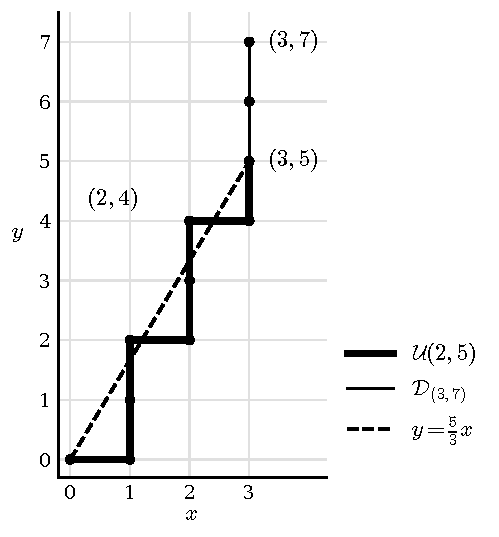
\includegraphics[height=66mm]{figures/example-2-19.pdf}
\caption{The thick line shows $\mathcal U(2,5)$. The thin line continues $\mathcal U(2,5)$ to
$\mathcal D_{(3,7)}$. The dashed segment joins $(0,0)$ to $(3,5)$.}
\label{fig:example-run}
\end{figure}
\end{example}

